The field of biology is changing rapidly from a qualitative
discipline to one rooted in quantitation.  These changes are driven
by advances in microfabrication and microelectronics that continue
to yield ever more creative ways to probe cellular function. These
advances, in turn, are producing a deluge of data, opening up new
ways to think about and analyze life, and attracting engineers and
scientists from other disciplines into biology.

Nowhere is this sea change of quantitation more pronounced than in
DNA sequencing~\cite{shendure2004advanced}.  As shown in
Figure~\vref{fig:moore}, improvements in DNA sequencing drove down
the cost of sequencing many orders of magnitude over the past 30
years, making sequencing commonplace.  This rate of sequencing
produces a data storage nightmare --- each dry gram of DNA can store
approximately a zettabyte of information, or a million million
gigabytes~\cite{reif2002computing}.  Consider the growth of the
Genbank DNA database~\cite{benson2006genbank}, as shown in
Figure~\vref{fig:moore}.  Genbank receives over 1000 new submissions
of DNA sequences from scientists every day and has doubled in size
every 18 months since 1982.

            \begin{figure}[ptb]
            \centering
            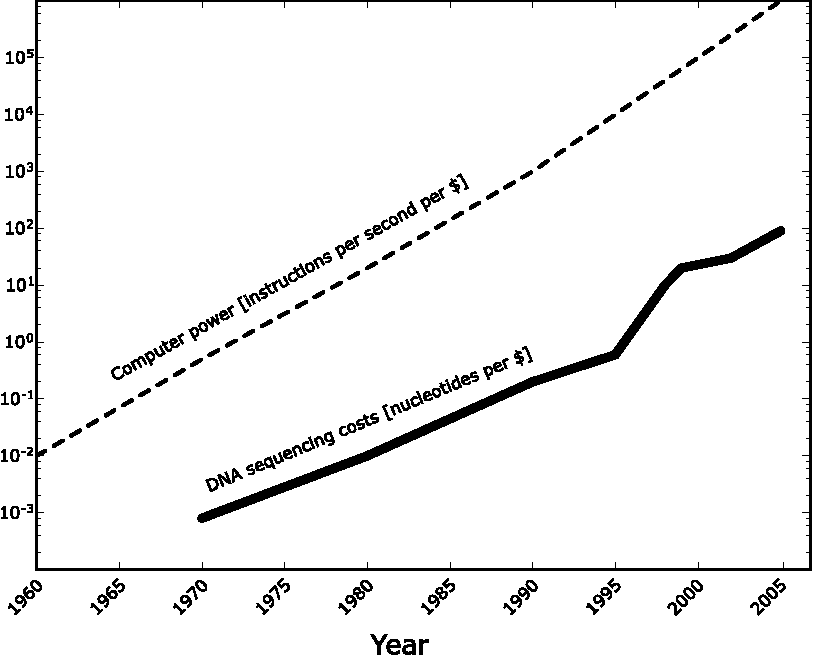
\includegraphics[width=\textwidth]{Body/Images-chap1/moore.pdf}
            \caption[Exponential growth of sequencing throughput]{
                Exponential growth of sequencing throughput~\cite{shendure2004advanced}.  The
                figure tracks the number of nucleotides that can be
                sequenced for a dollar over time juxtaposed with the
                advancement of computing power.  The hypothesis
                referred to as ``Moore's Law'' --- that
                computational power doubles every 18 months ---
                appears somewhat applicable to DNA sequencing.
                Engineering advancements in the basic
                electrophoretic method of DNA sequencing, the
                so--called ``Sanger sequencing,'' over the past 30 years
                decreased the cost of sequencing many--fold.  During
                the 15 year Human Genome Project, widespread
                investment into innovation and automation drove down the
                cost tenfold, greatly accelerating
                the completion of the project ---
                85\% of the genome was sequenced in the project's last
                two years~\cite{collins2003human}.
        }
            \label{fig:moore}
            \end{figure}

           \begin{figure}[ptb]
            \centering
            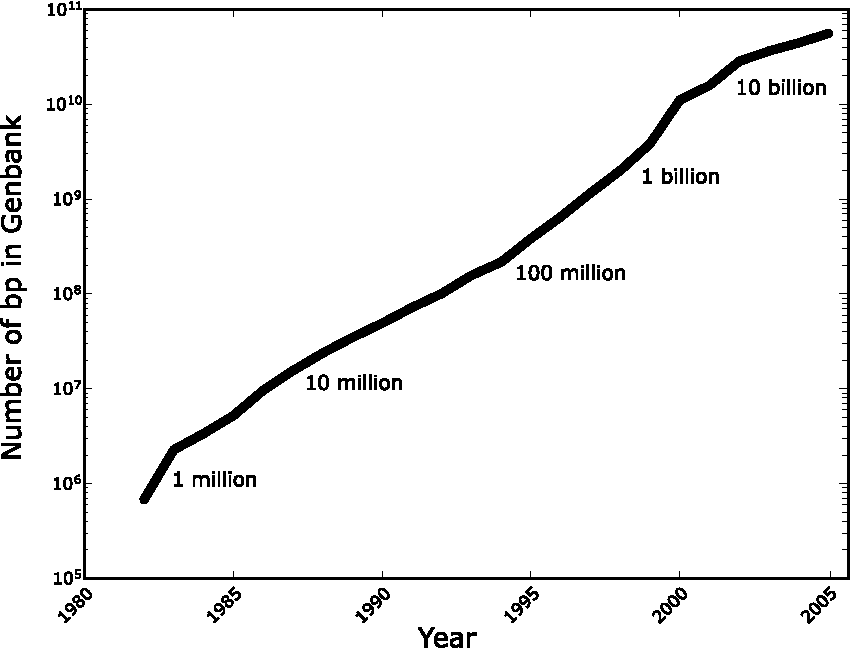
\includegraphics[width=\textwidth]{Body/Images-chap1/genbank.pdf}
            \caption[Exponential growth of Genbank]{Exponential
            growth of Genbank~\cite{benson2006genbank}.  Genbank is
            a comprehensive database of DNA sequences from over 200,000
            organisms that were made public by direct
            submission from researchers.  The database is maintained
            by the U.S. National Center for Biotechnology Information, and is updated daily.  The sequences in Genbank
            include data from genome sequencing projects, expressed
            sequence tags, and international sequence data from the
            European Molecular Biology Laboratory and the DNA
            Databank of Japan.  Genbank receives over 1000
            submissions per day and has doubled roughly every 18
            months since being started.  It is the largest database
            of its kind and is the basis for many
            ``information--added'' databases and resources.
            See also~\vref{fig:moore}.
        }
            \label{fig:genbank}
            \end{figure}


This torrent of data is not restricted to DNA sequencing.
Technological advances in recent years produced myriad tools
for quantifying biology including DNA microarrays, reverse
transcriptase polymerase chain reaction (RT--PCR), flow cytometry,
chromatin--immunoprecipitation (chip--chip), yeast two--hybrid
assays, fluorescence and confocal microscopy, generalized robotic
screening methods, and countless others.  These tools enable the
continual coining of new ``omes'' such as the transcriptome,
proteome, and interactome --- high--throughput counterparts to
traditional areas of study in biology.  (See Figure~\vref{fig:omes}
and Table~\vref{table:omes}.)  These new fields do not exist in
isolation, but instead contribute to an ever--increasing network of
information.  Consider the Genbank annotation of the human insulin
gene as shown an Figure~\vref{fig:genbank-record}. The annotation
includes detailed information about insulin culled from the
scientific literature by human experts including not just the
sequence of the gene, but also its post--translational
modifications, cellular localization, interactions with other genes,
role in energy metabolism and diabetes, and numerous links to
external databases with yet more information.

            \begin{figure}[ptb]
            \centering
            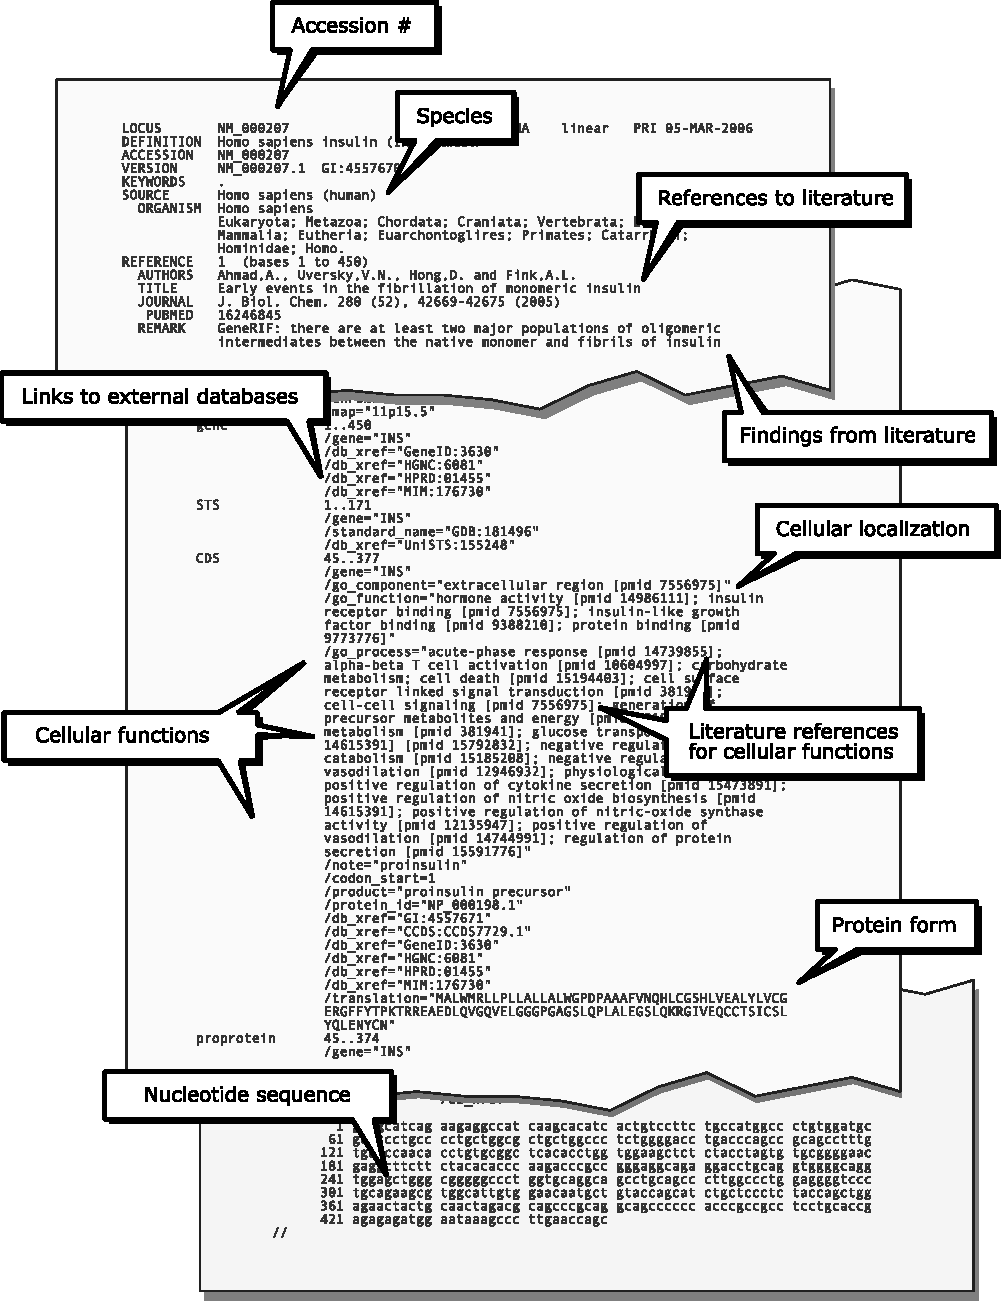
\includegraphics[width=0.90\textwidth]{Body/Images-chap1/genbank-record.pdf}
            \caption[A sample Genbank record]{A sample Genbank
            record showing the litany of features annotating the
            human gene for insulin.  As the figure suggests, this
            ``extra'' information typically dwarfs the gene sequence
            in size.  The annotations are highly cross--referenced,
            linking genes to cellular functions, behaviors,
            localizations and to other databases with yet more
            information.  Viewed \emph{en masse}, a complex network
            of knowledge emerges linking primary sequences
            into the understanding of higher--order systems at the
            cellular, tissue, an organism levels.
        }
            \label{fig:genbank-record}
            \end{figure}







\begin{table}
    \caption[``Omic'' fields other than genomic and proteomic]{
        ``Omic'' fields other than genomic and proteomic.
        In many cases, fields have been reborn as ``omic''
        fields due to a changing focus towards higher throughput
        empirical methods.  This list is indicative of the shift
        in biology towards quantitation and the resulting need
        for new, automated modes of analysis.  The rise
        of these words over time in the scientific vernacular
        is shown in Figure~\vref{fig:omes}.
        This list
        was compiled by searching over 5 million articles in the
        life sciences literature using the NCBI eutils
        API~\cite{ncbi2005eutils}.
        See also references in the
    bibliography~\cite{gerstein2005omes,dana2005omics}.
        }\label{table:omes}
	\centering
    \begin{tabular}{llll} \hline \hline
    Anatomics
    & Biomics
    & Chromosomics
    & Cytomics \\
     Enviromics
    & Epigenomics
    & Fluxomics
    & Glycomics \\
     Glycoproteomics
    & Immunogenomics
    & Immunomics
    & Immunoproteomics \\
     Integromics
    & Interactomics
    & Ionomics
    & Lipidomics \\
     Metabolomics
    & Metabonomics
    & Metagenomics
    & Metallomics  \\
     Metalloproteomics
    & Methylomics
    & Mitogenomics
    & Neuromics \\
     Neuropeptidomics
    & Oncogenomics
    & Peptidomics
    & Phenomics  \\
     Phospho-proteomics
    & Phosphoproteomics
    & Physiomics
    & Physionomics  \\
     Post--genomics
    & Postgenomics
    & Pre--genomics
    & Rnomics \\
     Secretomics
    & Subproteomics
    & Surfaceomics
    & Syndromics \\
     Transcriptomics \\ \hline \hline
    \end{tabular}
\end{table}



\begin{figure}
    \centering
    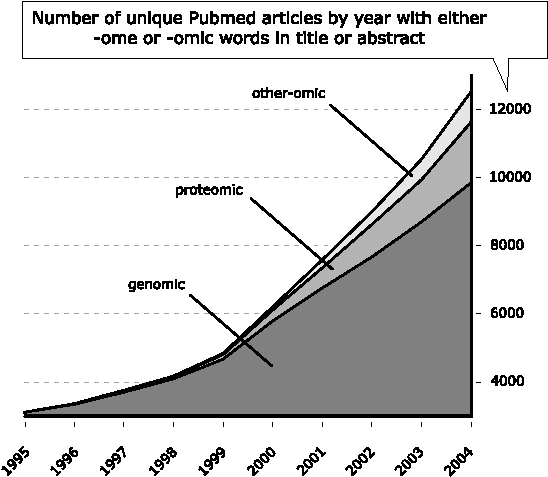
\includegraphics[width=0.8\textwidth]{Body/Images-chap1/omes.pdf}
    \caption[Usage of ``ome'' and ``omic'' words over time]{
            Usage of ``ome'' and ``omic'' words over time divided
            into three catagories: genome and genomic, proteome
            and proteomic, and other ome and omic.  The latter
            category comprises those words shown in
            Table~\vref{table:omes}.
    }\label{fig:omes}
\end{figure}



The Genbank annotation of insulin is the rule rather than the
exception.  It is a small piece of the growing wealth of data
describing life processes from the molecular level all the way to
the organism and ecological levels.  However, inasmuch as these data
hold promise, they also present challenges: if our ability to
collect data has increased exponentially, has our ability to
interpret and derive meaningful conclusions from these data kept
track? Will these diverse data allow us to ``connect the dots,'' to
reveal rich systems--level information? Or, instead, are they
subject to the law of diminishing returns? The prevailing punditry
lends credence to the former: witness the rise of systems
biology~\cite{ideker2003building,hwang2005data,salazar2006bioinformatics}.

But the problem remains: how can the potential of these volumous and diverse data sets
be realized?  The sheer amount of data points to the need for
automated, computational methods for analysis.  This need is driving
the co--opting of computer science as a core discipline of biology.
That is, computational methods are becoming increasingly necessary
to analyze the vast data sets biologists have accrued, and
consequently, computer science and mathematics are becoming as
fundamental to biology as chemistry and physics.  The particular
sub--discipline of biology devoted to these computational methods is
typically referred to as either bioinformatics or computational
biology.  Together, these fields comprise many research topics
devoted to both data analysis and modeling of biological systems.

It is likely that the need for automated, computational analysis
will only increase in the future. There are 334 completely sequenced
genomes and over 700 genomes in various stages of completion in the
genome database at the U.S. National Center for Biotechnology
Information (NCBI)~\cite{wheeler2006database}. But, of the finished
genomes, only two are mammalian: \emph{Homo
sapiens}~\cite{venter2001sequence,lander2001initial} and \emph{Mus
musculus}~\cite{waterston2002initial}, human and mouse. This
suggests that, rather than being in the ``post--genomic'' age, we
have just begun the genomic age. Upcoming years will see the
completion of many genomes with relevance to human health and
disease --- such as the rat, rabbit, and chimpanzee genomes --- and
to industry such as the cow, corn, and potato genomes.  Furthermore,
these are just the sequencing data.  Analogous progress in fields
such as metabolomics and proteomics is likely to leave biologists
awash in data, further exacerbating the need for automated methods
of interpreting and modeling these data.


The motivation for automated data analysis techniques that I have
painted in this introduction is quite broad, but what remains of
this thesis is not. The focus of the remainder is automated,
computational methods for discovering motifs in sequential data such
as DNA and protein sequences.  For example, imagine a scenario in
which we would like to correlate one of the annotations of insulin
shown in Figure~\ref{fig:genbank-record} to a particular part of the
DNA that encodes insulin. This is a very common problem in
bioinformatics.  In essence, this is like trying to learn a language
we don't speak by reading many books.  As suggested by
Figure~\vref{table:arabGenes}, this is a nontrivial problem.


                \begin{table}[!hbtp]
                \centering
                \caption[Gene sequences from \emph{Arabodopsis thaliana}]{Genes sequences from \emph{Arabodopsis thaliana},
                a popular plant model organism.  These very small genes are only a
                few hundred bases long, whereas a typical gene can be many kilo--bases in length.
                Given these sequences, how can we find all the small repeated
                motifs such as \texttt{CCACGCGTCCGAAAA}?  At a glance, the task seems
                difficult.
                Digging further it seems insurmountable --- the
                sequences below are just a small snippet of Genbank .  To
                print just the nucleotide sequences in Genbank
                using this font would require 30 million pages: a stack of
                paper 3 km high, or roughly the distance from MIT to
                Harvard.}\label{table:arabGenes}
                    \begin{tabular}{l}\hline\hline
$>$gi$\|$8571926 Arabidopsis thaliana lipid transfer protein \\
\ttfamily \footnotesize CCACGCGTCCGAAAAAAAAAACAGAAAGTAACATGAGATCTCTCTTATTAGCCGTGTGCCTGGTTCTTGC \\
\ttfamily \footnotesize TTTACACTGCGGTGAAGCAGCCGTGTCTTGCAACACGGTGATTGCGGATCTTTACCCTTGCTTATCCTAC \\
\ttfamily \footnotesize GTGACTCAGGGCGGACCGGTCCCAACCCTCTGCTGCAACGGTCTCACAACACTCAAGAGTCAGGCTCAAA \\
\ttfamily \footnotesize CTTCTGTGGACCGTCAGGGGGTCTGTCGTTGCATCAAATCTGCTATTGGAGGACTCACTCTCTCTCCTAG \\
\ttfamily \footnotesize AACCATCCAAAATGCTTTGGAATTGCCTTCTAAATGTGGTGTCGATCTCCCTTACAAGTTCAGCCCTTCC \\
\ttfamily \footnotesize ACTGACTGCGACAGTATCCAGTGAGACAAGCAGAAAATCTTAAAGGAAGCTACTACAAGAACTATAATAA \\
\ttfamily \footnotesize CCTAATAATTAATAAATGAGGGCATTGGTTTGCTAGTTGCTAATTGATCAGTGATGTATTGTCATTTTGA \\
\ttfamily \footnotesize ATGTTCTAATATCAGCAGGCACTTATCTCTGAAAAAAAAAAAAAAAA \\ \\
$>$gi$\|$8571922 Arabidopsis thaliana lipid transfer protein \\
\ttfamily \footnotesize CCACGCGTCCGAAAACACAAGCGTAGAAAACAAAACTCAACTAATTGTGTTATCACCCAAAAGAGAAGAG \\
\ttfamily \footnotesize CAAACACAATGGCTTTCGCTTTGAGGTTCTTCACATGCTTTGTTTTGACAGTGTTCATCGTTGCATCAGT \\
\ttfamily \footnotesize GGATGCAGCAATAACATGTGGCACAGTGGCAAGTAGCTTGAGTCCATGTCTAGGCTACCTATCGAAGGGT \\
\ttfamily \footnotesize GGGGTGGTGCCACCTCCGTGCTGTGCAGGAGTCAAAAAGTTGAACGGTATGGCTCAAACCACACCCGACC \\
\ttfamily \footnotesize GCCAACAAGCATGCAGATGCTTACAGTCCGCTGCAAAAGGGGTTAATCCAAGTCTAGCCTCTGGCCTTCC \\
\ttfamily \footnotesize TGGAAAGTGCGGTGTTAGCATCCCCTATCCCATCTCCACGAGCACCAACTGCGCCACCATCAAGTGAAGT \\
\ttfamily \footnotesize GGGGAATAACGACATCATTTGCCTGAAGAGTATGGTTTCGTATACGTAAAATAAGACGGCTATCTAAGCT \\
\ttfamily \footnotesize GATATTTACCTTGTCTTTGTTTGTCTTGATGGCTTTGTAATCTTTTGCTTTGTTATGTTGTATACTTGTG \\
\ttfamily \footnotesize TCTTAACATGTTTAAGATATGATAATATATAGTATCGGTACCTTATTAAAAAAAAAAAAAAA \\ \\
$>$gi$\|$8571922 Arabidopsis thaliana lipid transfer protein \\
\ttfamily \footnotesize CCACGCGTCCGAAAACACAAGCGTAGAAAACAAAACTCAACTAATTGTGTTATCACCCAAAAGAGAAGAG \\
\ttfamily \footnotesize CAAACACAATGGCTTTCGCTTTGAGGTTCTTCACATGCTTTGTTTTGACAGTGTTCATCGTTGCATCAGT \\
\ttfamily \footnotesize GGATGCAGCAATAACATGTGGCACAGTGGCAAGTAGCTTGAGTCCATGTCTAGGCTACCTATCGAAGGGT \\
\ttfamily \footnotesize GGGGTGGTGCCACCTCCGTGCTGTGCAGGAGTCAAAAAGTTGAACGGTATGGCTCAAACCACACCCGACC \\
\ttfamily \footnotesize GCCAACAAGCATGCAGATGCTTACAGTCCGCTGCAAAAGGGGTTAATCCAAGTCTAGCCTCTGGCCTTCC \\
\ttfamily \footnotesize TGGAAAGTGCGGTGTTAGCATCCCCTATCCCATCTCCACGAGCACCAACTGCGCCACCATCAAGTGAAGT \\
\ttfamily \footnotesize GGGGAATAACGACATCATTTGCCTGAAGAGTATGGTTTCGTATACGTAAAATAAGACGGCTATCTAAGCT \\
\ttfamily \footnotesize GATATTTACCTTGTCTTTGTTTGTCTTGATGGCTTTGTAATCTTTTGCTTTGTTATGTTGTATACTTGTG \\
\ttfamily \footnotesize TCTTAACATGTTTAAGATATGATAATATATAGTATCGGTACCTTATTAAAAAAAAAAAAAAA \\\hline\hline
\end{tabular}

                \end{table}

Motif discovery in sequential data is only one tiny sliver of the
vast spectrum of topics spanned by bioinformatics and computational
biology. However, many of the principles and tools I describe have
broader implications for learning and automated discovery methods in
biology.  Chapter 1 of this thesis is devoted to familiarizing the
reader with basic concepts of motif discovery, with a particular
focus on linguistic methods of modeling sequences. In Chapter 2,
these concepts are applied to the annotation and design of novel
antibiotics, called antimicrobial peptides.  The principal
contribution of this thesis is the third chapter, in which I develop
a framework and software tool for motif discovery that can be
generalized to diverse types of data and is superior to existing
tools in many ways.  Finally, the last chapter comprises a series of
vignettes that take a more broad approach to motif discovery and
explore a number of issues adjoining the central theme of the first
three chapters.

\section{Fundamental tenets of motif discovery}\label{section:tenents}

I will begin with a series of elementary, almost philosophical
examples that serve to illustrate some of the fundamental tenets of
motif discovery. These examples may seem pedantic; however, the
tenets they illustrate will be recurring themes throughout this
thesis. Further, the following sections will serve to establish a
common vocabulary and mode of thought that will enable the
development of more complex ideas in later chapters.

In the most basic sense, the task of motif discovery is to find a
repeated feature in a data set.  Take, for example, the objects below.


\begin{equation}\label{eqn:shapes}
    \blacksquare\blacktriangle\square\blacksquare
\end{equation}



What features are repeated at least twice in the objects?  One
answer is that the square shape appears three times.  Yet another,
is that three of the objects are darkened.  And finally, a more
sophisticated answer is that all of the objects are regular
polyhedrons.  Which of these is correct? All three are.  The first
two answers are intuitively obvious, whereas the final answer is
rooted in a knowledge of geometry.  The degree to which one answer
is ``more correct'' than the others depends on what kinds of
features we are interested in \emph{a priori}.  This is the first
and most important tenet of motif discovery.


Consider a second question: is the dark square more similar to the
dark triangle or to the hollow square?

\begin{equation}\label{eqn:shapes2}
    \blacksquare\sim\blacktriangle\sim\square
\end{equation}

Again, there is no correct answer. The response obviously depends on
our relative preference for color versus shape.  This variety of
question is even more difficult when we seek to quantify the degree
of similarity or difference --- the distance --- between two
objects.  Is a human more similar to an alligator, or to an
elephant? Based on body temperature, the human is more similar to
the elephant; however, based on weight, the opposite true.  This is
the second tenet of motif discovery: the measurement of
``distance'' between objects is inherently relative, or dependent on
predefined metrics.

Now consider a more complicated example shown schematically in
Figure~\vref{fig:gaussian}.  The figure shows an X--Y scatter plot
with 12 data points.  How many groups of points, or clusters, are in
this figure?  As before, there are many correct answers: three
groups of four; one group of four and one group of eight; or one
single group of twelve.  The answer depends on our preconceived
notion of how small the distance between objects must be in order
for them to be grouped together.  Or, equivalently, how similar
objects must be to be considered the same.  This is our third and final
tenet of motif discovery.

            \begin{figure}[ptb]
            \centering
            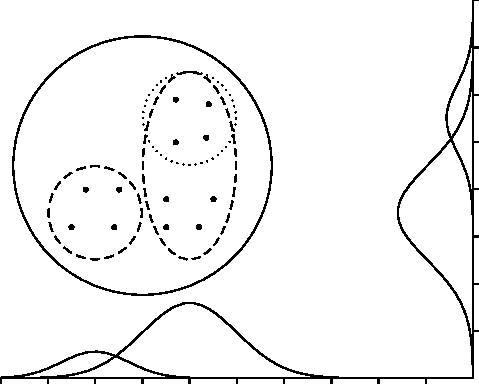
\includegraphics[width=\textwidth]{Body/Images-chap1/gaussian.pdf}
            \caption[Finding patterns in generic data]{Clustering to find patterns in generic data.  Given this data set,
            we would cluster the data together to find patterns (indicated here by the ellipses).  But, there are many different
            patterns we could find.  Which ones are correct?}
            \label{fig:gaussian}
            \end{figure}

The three tenets we have just developed can be rephrased as follows.
The answer to any motif discovery problem will always depend on what
kinds of motifs we are looking for and the search for these motifs
will always depend on a predefined metric of similarity and method
for grouping together similar objects.

\section{Motif discovery in sequential data}


In this section, I define ``sequential data'' and introduce some
basic concepts of motif discovery in sequential data.  I will build
upon tenets developed in the previous section and develop more
complex ideas in motif discovery that are specific to sequential
data.

In the most general sense, sequential data are any data in which
there is a natural ordering, such that rearranging the data would
result in lost information.  In later chapters, we will deal with
the more general case of sequential data that encompasses series of
multidimensional real--valued data; however, for the time being, we
can consider sequential data to be a series of alphanumerical
characters such as the four sequences shown below.

\begin{multline}\label{eqn:lincoln1}
   \texttt{djndfduckdeicfjnfmABRAHAMLINCOLN}\\
   \texttt{idkeioddsnABRAHAMLINCOLNaknkwbad}\\
   \texttt{ioxcABRAHAMLINCOLNabkjwlkdaxlakj}\\
   \texttt{xkasnkjlfABRAHAMLINCOLNkdsjkjsdl}
\end{multline}



    We can refer to these sequences more formally by calling the set
    of sequences $S$, where $S$ is defined such that
     $S=\braces{s_0,s_1,s_2,\ldots,s_n}$, and where
    sequence $s_i$ has length $W_i$.  So, in the above example, $n=3$
    and $s_0=\texttt{djndfduckdeicfjnfmABRAHAMLINCOLN}$.  Furthermore, let
    the
    the $\ith{j}$ member of the $\ith{i}$ sequence
    be denoted by $s_{i,j}$.
    So, $s_{0,0}=d$, $s_{0,1}=j$, etc.
    Each $s_{i,j}$ is a
    primitive, or atomic unit, for the data that is
    being analyzed.  For now, we will say that the primitives
    are alphanumerical characters selected from some alphabet
    $\Sigma$.  In the example above, this alphabet is the set of 52
    lowercase and uppercase characters from the Roman alphabet.
    However, this alphabet can be defined in many different ways
    depending on the context of our motif discovery problem.  For
    example, for a DNA sequence the alphabet would
    comprise the characters $\{\texttt{A,T,G,C}\}$, representing the
    four bases found in DNA: adenosine, thymine, guanine, and
    cytosine (see Figure~\vref{fig:bases} in the Appendix.  Or, for protein sequences,
    the alphabet would be the
    set of characters representing the one letter abbreviations for
    the 20 naturally occurring amino acids
    $\{\texttt{A,R,N,D,C,Q,E,G,H,I,L,K,M,F,P,S,T,W,Y,V}\}$, which
    are defined in Figure~\vref{fig:aas} in the Appendix.


In the set of sequences above, the motif ``\texttt{ABRAHAMLINCOLN}''
is inherently obvious in the otherwise random series of characters
that make up each of the individual sequences.  A similar motif is
obvious even when the sequences are ``mutated'' as shown below.



\begin{align}\label{eqn:lincoln2}
   s_0 &= \texttt{djndfduckdeicfjnfmABELINCOLN}\\
   s_1 &= \texttt{idkeioddsnABRAHAMLINCOLNaknkwbad}\notag\\
   s_2 &= \texttt{ioxcALINCOLNabkjwlkdaxlakj} \notag\\
   s_3 &= \texttt{xkasnkjlfABRAHAMLINCOLNkdsjkjsdl}\notag
\end{align}

In two of these sequences, Abraham is abbreviated but is still
recognizable.  But now, it is not appropriate to call the motif
simply ``\texttt{ABRAHAMLINCOLN}.''  At this point, it is important
to develop a more rigorous definition of ``motif'' that will allow
us to describe all the possible permutations shown in the above
mutated sequences.  A motif is, henceforth, a mathematical model
used to describe a set of locations in a set of sequences.  These
locations are referred to as ``motif instances.''  In the example
above, the motif instances are the substrings:
``\texttt{ABELINCOLN},'' ``\texttt{ABRAHAMLINCOLN},''
``\texttt{ALINCOLN},'' and ``\texttt{ABRAHAMLINCOLN}'' in sequences
$s_0$, $s_1$, $s_2$, and $s_3$, respectively.

Any mathematical model used to describe these instances should say
that each instance begins with the letter \texttt{A}, optionally
followed by either \texttt{BE} or \texttt{BRAHAM}, and necessarily
followed by \texttt{LINCOLN}.  That is, a model that describes the
ordered arrangement of objects, in this case characters.  Such
models are commonplace in the field of linguistics and are called
grammars.

\section{Grammatical models of sequences}


\subsection*{Introduction}

The theory underlying grammatical models of sequences can be traced
back to Noam Chomsky's early work on syntax
theory~\cite{chomsky1957syntactic,chomsky1965aspects,chomsky1956three}.
 Chomsky's work is the basis for much of formal language theory and
computational linguistics.  However, in general, most research in these
areas has used grammars for pattern \emph{recognition} vice pattern
\emph{discovery}, and focuses on machine learning techniques for
computer understanding of natural languages. Only recently have
these pattern recognition techniques been applied to problems of
interest to
biologists~\cite{searls1997linguistic,searls2001reading,searls1992thecomputational}.

As I will show in the following sections, most motif discovery
algorithms in bioinformatics use motif models that can be reduced,
in general, to a grammatical model.  However, for the most part,
such reductions are rare in the bioinformatics literature. This is
because motif discovery and bioinformatics evolved independently
from formal language theory.  In a sense, the two fields are distant
homologs of each other, both making use of models that can be
reduced to grammars.


A grammar is a mathematical construct that describes the ordered
arrangement of objects, usually words or characters, in a
sequence~\cite{aho1979theory}.
 More rigorously, a grammar is a 4--tuple $G = (N,\Sigma,P,S) $
 wherein
\begin{enumerate}\label{grammarDefinition}
  \item $N$ is a finite set of non-terminal symbols, also called
  variables or syntactic categories;
  \item $\Sigma$ is a finite set of terminal symbols, disjoint from
  $N$;
  \item $P$ is a finite subset of
    \begin{equation}\label{eqn:production}
        (N\cup\Sigma)*N(N\cup\Sigma)*\times(N\cup\Sigma)*,
    \end{equation}
    each element in $P$ is called a ``production'' and
    is written in the form $\alpha\rightarrow\beta$%
    \footnote{The star symbol, $*$, is called the Kleene star and is
    interpreted as ``zero or more'' of the expression it follows.
    For example, \texttt{ZA*} would be interpreted as a \texttt{Z}
    followed by zero or more \texttt{A} characters.  The Kleene star
    and other similar operators will be discussed later in the
    section on regular grammars and regular expressions\vref{section:regex}.
    }; and,
    \item $S$ is a special symbol in $N$ that is the start symbol.
\end{enumerate}

To illustrate how a grammar can be used to model sequences, consider
the following simple grammar:

\begin{equation}\label{eqn:simpleGrammar}
    G = (\{\alpha, S\},\{\texttt{0}, \texttt{1}\},P,S),
\end{equation}

where the set of productions, $P$, is given by

\begin{align}\label{eqn:simpleProduction}
    P =
    \begin{cases}
    S \rightarrow \texttt{0}\alpha \texttt{1}\\
    \texttt{0}\alpha \rightarrow \texttt{00}\alpha \texttt{1}\\
    \alpha \rightarrow e.
    \end{cases}
\end{align}

Each line in the set of productions is essentially a replacement
rule. For example, the operation $S \rightarrow \texttt{0}\alpha
\texttt{1}$ should be read as ``replace the character $S$ with the
sequence of characters $\texttt{0}\alpha \texttt{1}$.''  Then, the
subsequent line should be read as ``replace the two character
sequence $\texttt{0}\alpha$ with the sequence $\texttt{00}\alpha
\texttt{1}$.''  Finally, the last production should be read as
``replace the character $\alpha $ with the character $e$, which is
the termination character.''  These productions follow a few
conventions that are used throughout this manuscript.  First, as
defined on page~\pageref{grammarDefinition}, $S$ is a special
non--terminal symbol that is always used as the starting symbol.
Second, in order to distinguish terminal symbols from non--terminal
symbols, the former will always be displayed in a fixed width font.
Third, the
character $e $ is used always to represent the termination of a
sequence and is referred to as the termination character.

Now consider how to construct a sequence using the set of
productions in the grammar shown in
Equations~\ref{eqn:simpleGrammar} and~\ref{eqn:simpleProduction}.  Starting
with the special non--terminal character $S$, the first production
produces a three letter sequence.
\begin{align*}
    S &\Rightarrow \texttt{0}\alpha \texttt{1}
\end{align*}
Using the second production, produces a four character sequence.
\begin{align*}
    S &\Rightarrow \texttt{0}\alpha \texttt{1}  \Rightarrow \texttt{00}\alpha \texttt{1}
\end{align*}
Finally, using the third production terminates the sequence.
\begin{align}\label{eqn:simpleDerivation}
    S \Rightarrow \texttt{0}\alpha \texttt{1}  \Rightarrow \texttt{00}\alpha \texttt{1}
    \Rightarrow \texttt{001}
\end{align}

The sequences produced by following the production rules of the
grammar are called derivations of a grammar, or equivalently the
sentences or sentenial forms of the grammar.  The collection of
sentenial forms of a grammar are collectively called the language
generated by $G$, or $L(G)$.

Notably, the final sequence shown in
Equation~\ref{eqn:simpleDerivation} is not the only sequence that
can be derived from the grammar $G$.  Because the symbol
$\alpha$ appears in two different productions, either production can
be used and neither production is preferred \emph{a priori}.  For
example the following sequence is an equally valid derivation of the
same grammar.
\begin{align}\label{eqn:simpleDerivation2}
    S \Rightarrow \texttt{0}\alpha \texttt{1}  \Rightarrow \texttt{00}\alpha \texttt{1}
    \Rightarrow \texttt{000}\alpha \texttt{1}
    \Rightarrow \texttt{0000}\alpha \texttt{1}
    \Rightarrow \texttt{00000}\alpha \texttt{1}
    \Rightarrow \texttt{00000}\texttt{1}
\end{align}
As the derivation above suggests, any sequence that
\begin{itemize}
  \item begins with a \texttt{0},
  \item that is followed by zero or more \texttt{0}s, and
  \item is terminated by a single \texttt{1}
\end{itemize}
could be a derivation of the grammar shown in
Equation~\vref{eqn:simpleGrammar}. Collectively, these derivations
form the language of the grammar.


Now I will return to the Abraham Lincoln example shown in
Equation~\vref{eqn:lincoln2}.  Recall that the motif instances are
the substrings ``\texttt{ABELINCOLN},'' ``\texttt{ABRAHAMLINCOLN},''
``\texttt{ALINCOLN},'' and ``\texttt{ABRAHAMLINCOLN}'' in sequences
$s_0$, $s_1$, $s_2$, and $s_3$, respectively.  A grammar that
describes these motif instances is
\begin{equation}\label{eqn:abeGrammar}
    G = (\{\alpha, S\},\{\texttt{A}, \texttt{B}, \texttt{C},\texttt{E}, \texttt{H}, \texttt{I},
    \texttt{L}, \texttt{M}, \texttt{N}, \texttt{R}\},P,S),
\end{equation}
where $P$ is given by the set of productions
\begin{align}\label{eqn:abeProduction}
    P =
    \begin{cases}
    S \rightarrow \texttt{A}\alpha \\
    \alpha \rightarrow \beta \\
    \alpha \rightarrow \texttt{BE}\beta \\
    \alpha \rightarrow \texttt{BRAHAM}\beta \\
    \beta \rightarrow \texttt{LINCOLN}\gamma \\
    \gamma \rightarrow e.
    \end{cases}
\end{align}


Again, in a manner similar to Equation~\vref{eqn:simpleProduction},
the grammar shown in Equation~\vref{eqn:abeProduction} has a
non--terminal character, $\alpha$, in multiple productions.  In such
cases, the production can usually be abbreviated using the ``$\mid$''
character, which is to be read as ``or.''  For example, the
productions in Equation~\vref{eqn:abeProduction} can be written
equivalently as
\begin{align}\label{eqn:abeProduction2}
    P =
    \begin{cases}
    S \rightarrow \texttt{A}\alpha \\
    \alpha \rightarrow \beta \mid \texttt{BE}\beta \mid \texttt{BRAHAM}\beta \\
    \beta \rightarrow \texttt{LINCOLN}\gamma \\
    \gamma \rightarrow e.
    \end{cases}
\end{align}

Notice that the grammar shown in Equation~\vref{eqn:abeProduction}
describes exactly all four of the motif instances in the sequences
shown in Equation~\vref{eqn:lincoln2}.  The three possible
derivations of the grammar are shown below.
\begin{align}\label{eqn:abeDerivation}
    S \Rightarrow \texttt{A}\alpha   \Rightarrow \texttt{A}\beta
         \Rightarrow \texttt{ALINCOLN}\gamma  \Rightarrow
        \texttt{ALINCOLN}\\
    S \Rightarrow \texttt{A}\alpha   \Rightarrow \texttt{ABE}\beta
         \Rightarrow \texttt{ABELINCOLN}\gamma  \Rightarrow
        \texttt{ABELINCOLN}\notag\\
    S \Rightarrow \texttt{A}\alpha   \Rightarrow \texttt{ABRAHAM}\beta
        \Rightarrow \texttt{ABRAHAMLINCOLN}\gamma  \Rightarrow
        \texttt{ABRAHAMLINCOLN}\notag
\end{align}

This is an ideal case.  In general, in constructing any model
describing any motif instances, we would like to use a grammar that
is sensitive for the instances
--- i.e.\ all the instances are derivations of $G$ --- and specific
for the instances --- i.e.\ the language $L (G)$ includes few
derivations that are not motif instances.

Now consider a more complicated case in which a grammar is used to
model DNA sequences that are likely to assume a hairpin structure,
such as those shown in Figure~\vref{fig:hairpin}.  Hairpins in DNA
and RNA sequences play an important role in the regulation of many
processes, including transcription and translation.  A hairpin is
essentially a structure that bends back upon itself and is held
together by Watson--Crick pairing.  The paired bases in the hairpin
structure are referred to as the ``stem'' and the unpaired, bulging
bases are referred to as the ``loop'' (see
Figure~\vref{fig:hairpin}).

            \begin{figure}[ptb]
            \centering
            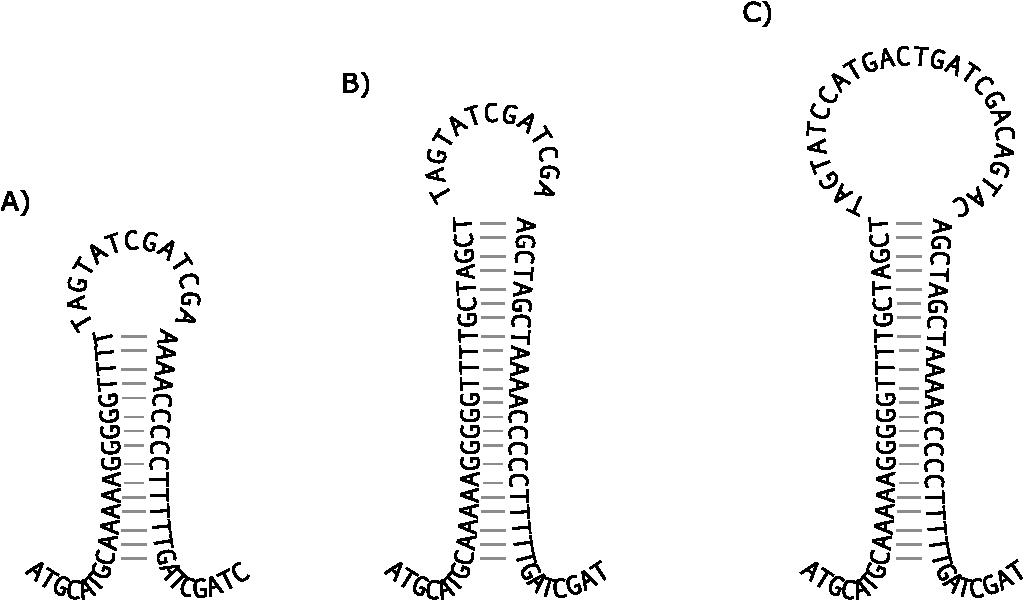
\includegraphics[width=\textwidth]{Body/Images-chap1/hairpin.pdf}
            \caption[Hairpin loops in DNA secondary structures]{
            Hairpin loops in DNA secondary structures.  A hairpin
            loop is a secondary structure in a sequence containing two
            regions that are reverse complements of each other.
            These regions form the ``stem'' of the hairpin loop.
            The figure shows three hairpin loops in which the stem
            size gets progressively larger.  Also notice that, the
            bulbous region --- the ``loop'' --- which is not paired
            with any other region, can be of arbitrary size.  The
            structures play an important part in the regulation of
            DNA transcription and, for RNA, in the process of
            translation.
            }
            \label{fig:hairpin}
            \end{figure}

In order to form a stem--loop, or hairpin structure, the two
sequences in the stem must be reverse complements of each other.
This type of relationship is captured in the following grammar:
\begin{equation}\label{eqn:hairpinGrammar}
    G = (\{\alpha, \beta, S\},\{\texttt{A}, \texttt{G},\texttt{T},\texttt{C}\},P,S),
\end{equation}
where $P$ is given by
\begin{align}\label{eqn:hairpinProduction}
    P =
    \begin{cases}
    S \rightarrow \alpha \\
    \alpha \rightarrow \texttt{A}\alpha\texttt{T} \mid \texttt{T}\alpha\texttt{A} \\
    \alpha \rightarrow \texttt{G}\alpha\texttt{C} \mid \texttt{C}\alpha\texttt{G} \\
    \alpha \rightarrow \beta \mid e \\
    \beta \rightarrow \texttt{A}\beta \mid \texttt{T}\beta \mid\texttt{G}\beta \mid
        \texttt{C}\beta \mid e
    \end{cases}
\end{align}


The grammar shown in Equation~\vref{eqn:hairpinGrammar} can describe
any hairpin loop in which the stem consists of one or more
complementary bases and the loop consists of zero or more bases.  For
example, consider the following derivation of the grammar.
\begin{equation}\label{eqn:hairpinDerivation}
\begin{split}
    S &\Rightarrow \alpha \\
    &\Rightarrow \texttt{A}\alpha\texttt{T} \\
        &\Rightarrow \texttt{AG}\alpha\texttt{CT} \\
        &\Rightarrow \texttt{AGG}\alpha\texttt{CCT} \\
        &\Rightarrow \texttt{AGGC}\alpha\texttt{GCCT} \\
        &\Rightarrow \texttt{AGGCT}\alpha\texttt{AGCCT} \\
        &\Rightarrow \texttt{AGGCT}\beta\texttt{AGCCT} \\
        &\Rightarrow \texttt{AGGCTA}\beta\texttt{AGCCT} \\
        &\Rightarrow \texttt{AGGCTAAGCCT}
\end{split}
\end{equation}
This derivation produces a sequence that can form a hairpin
structure with a stem size of five base pairs and a loop of a single
base pair.

The grammar shown in Equation~\vref{eqn:hairpinGrammar} is more
complex than the grammar used to model the Abraham Lincoln motif
(Equation~\vref{eqn:abeGrammar}), because there are a long--range
dependencies in the sequences.  That is, a particular base produced
by the grammar in Equation~\ref{eqn:hairpinGrammar} is guaranteed
to be complementary to a base on the other side of the sequence.  In
contrast, the productions used to model the Abraham Lincoln motif
produced a set of simple derivations in a left--to--right order.
Indeed, even more complicated grammars can describe still more
long--range, complex interactions between the characters in a
sequence.


\subsection*{Hierarchy of restricted grammars}

Linguists classify grammars into four increasingly complicated
groups based on the format of their productions.  A grammar is
\begin{enumerate}
  \item right--linear, or type--3, if each production in $P$ is of the form
        $A\rightarrow \texttt{x}B$, where $A$ and $B$ are in  $N$
        and $\texttt{x}$ is any string in $\Sigma*$;\label{gramDefs}
  \item context--free, or type--2, if each production in $P$ is of the form
        $A\rightarrow \alpha$, where $A$ is in  $N$
        and $\alpha$ is  in $(N\cup\Sigma)*$;
  \item context-- sensitive, or type--1, if each production in $P$ is of the form
        $\alpha A\beta \rightarrow \delta y \Gamma$, where $A$ is in  $N$,
        $y$ is non--null, and $\alpha$,
        $\beta$, $\delta$, and $\gamma$ are  in $(N\cup\Sigma)*$;
  \item unrestricted, or type--0, if it adheres to none of these
        restrictions.
\end{enumerate}
This classification system is referred to as the Chomsky
hierarchy~\cite{chomsky1956three}. Each of these grammars defines a
corresponding class of language, which is the set of all sequences
that can be produced using a particular type of grammar.

Right--linear, or type--3 grammars are also called ``regular''
grammars and are the simplest type of grammar. These grammars are
called right--linear because derivations of these grammars are
produced stepwise from left to right, never growing from the center
of the sequence as in the derivation shown in
Equation~\ref{eqn:hairpinDerivation}.  As I will show in
Section~\vref{section:regex}, despite their simplicity, regular
grammars are the most frequently used motif model in bioinformatics.

Context--free grammars are the next most complicated class of
grammatical model.  Indeed, the hairpin grammar shown in
Equation~\vref{eqn:hairpinGrammar} is a context--free grammar.  This
type of grammar is characterized by ``nested'' dependencies (see
Figure~\ref{fig:dependencies}).  The dependencies are nested in the
sense that derivations of the grammar ``grow'' from the center, due
to the structure of the productions.


            \begin{figure}[ptb]
            \centering
            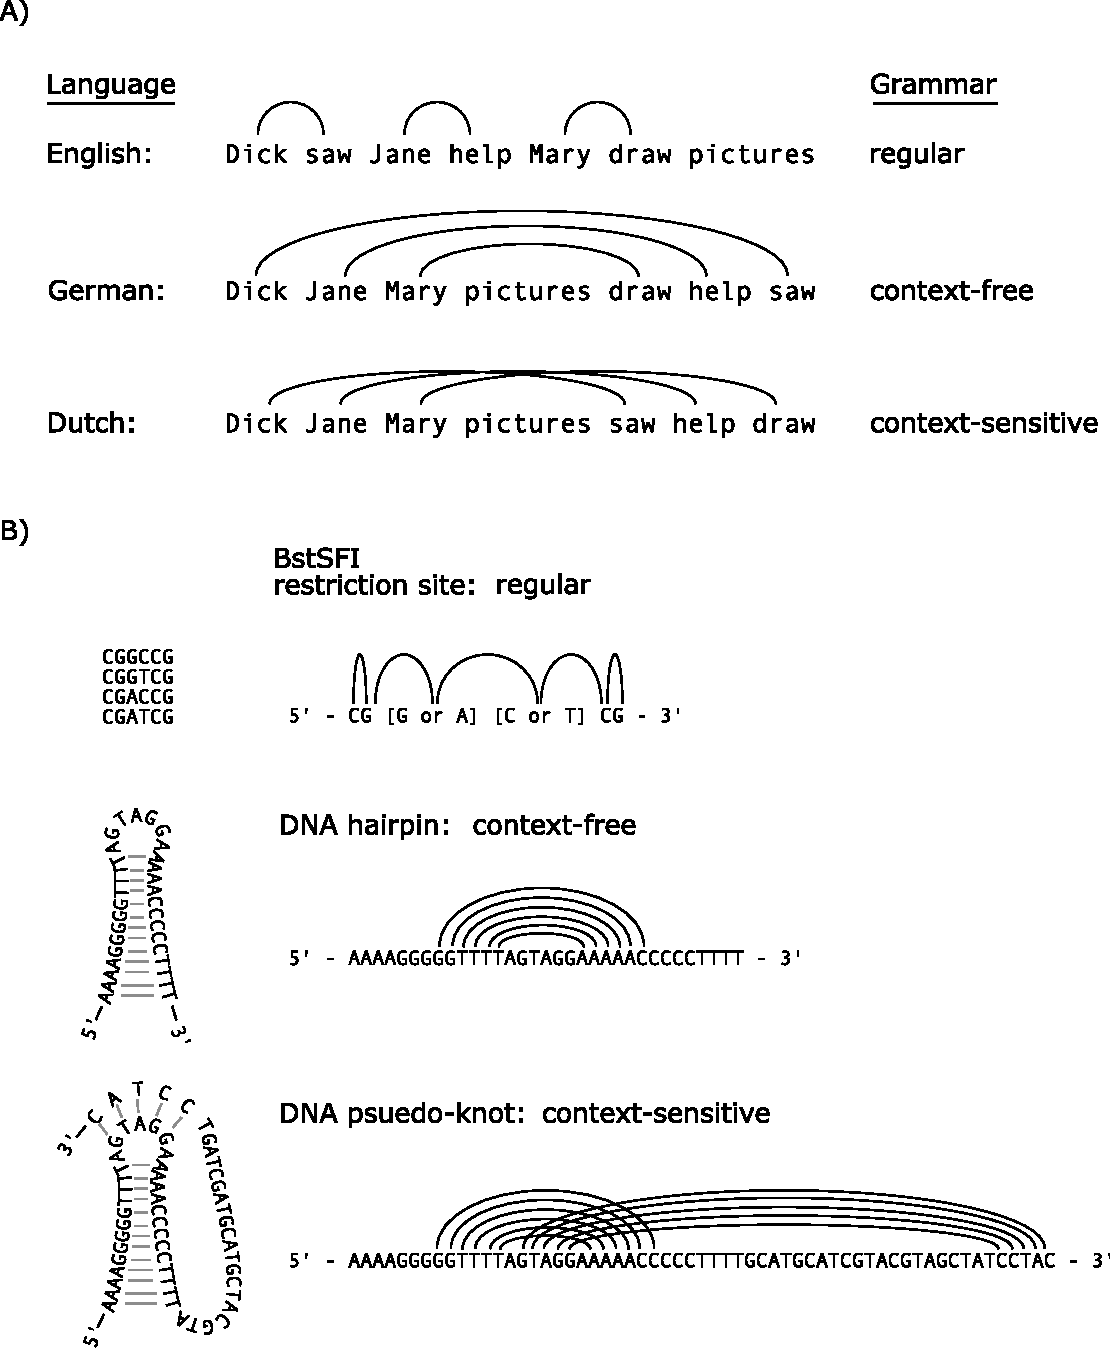
\includegraphics[width=0.80\textwidth]{Body/Images-chap1/dependencies.pdf}
            \caption[Noun--verb dependencies in various languages and their
            biological analogues]{Noun--verb dependencies in various languages and their
            biological analogues.  Part A) shows the sentence
            ``Dick saw Jane help Mary draw pictures'' translated
            grammatically into German and Dutch.  That is, the words
            in the sentence are rearranged to reflect the rules of
            grammar in these two languages, but the sentence is not
            translated \emph{per se}.  As shown, the English
            version of the sentence has a relatively simple
            dependency structure between the nouns and verbs that
            can be modeled using regular grammars.  In contrast,
            German and Dutch require more complicated grammatical
            models~\cite{shieber1985evidence,bresnan1982cross,jurafsky2000speech}.
            Part B) shows the biological analogue of the three
            sentences in Part A).  Typically, restriction sites can
            be modeled using regular grammars, whereas complex DNA
            secondary structures require context--free or
            context--sensitive grammars~\cite{rivas2000language}.  In the first example, the
            arches are used to represent a ``must be followed by''
            dependency.  In the second two examples, they represent
            a ``must be complementary to'' dependency.
            }
            \label{fig:dependencies}
            \end{figure}

Context--sensitive grammars and unrestricted grammars are the most
complex classes of grammatical models.  As shown in
Figure~\vref{fig:dependencies}, context--sensitive grammars are
characterized by long--range dependencies that are ``crossing.''
Derivations of these grammars can typically ``grow'' from anywhere
inside the sequence.  For example, consider the following grammar
that describes a card player arranging a deck of cards:
\begin{equation}\label{eqn:csGrammar}
    G = (\{\gamma, \beta, S\},\{\clubsuit, \heartsuit, \spadesuit\},P,S),
\end{equation}
where $P$ is given by
\begin{align}\label{eqn:csProduction}
    P =
    \begin{cases}
    S \rightarrow \gamma \\
    \gamma \rightarrow \clubsuit\heartsuit\spadesuit \mid \clubsuit\gamma\beta\spadesuit \\
    \spadesuit\beta \rightarrow \beta\spadesuit \\
    \heartsuit\beta \rightarrow \heartsuit\heartsuit
    \end{cases}
\end{align}

This grammar is one of the most simple context--sensitive grammars.
As well, it serves to illustrate that sequential data are not
restricted to characters \emph{per se}.  Indeed, in
Chapter~\vref{chapter:gemoda}, I will extend the definition of
sequential data to include ordered arrangements  of multidimensional
real--valued data sampled from a continuous distribution.  Returning
to the current example, consider the following derivation of this
grammar:
\begin{equation}\label{eqn:csDerivation}
    \begin{split}
    S &\Rightarrow \gamma  \\
        &\Rightarrow \clubsuit\gamma\beta\spadesuit \\
        &\Rightarrow \clubsuit\clubsuit\gamma\beta\spadesuit\beta\spadesuit \\
        &\Rightarrow \clubsuit\clubsuit\clubsuit\gamma\beta\spadesuit\beta\spadesuit\beta\spadesuit \\
        &\Rightarrow \clubsuit\clubsuit\clubsuit\clubsuit\heartsuit\spadesuit\beta\spadesuit\beta\spadesuit\beta\spadesuit \\
        &\Rightarrow \clubsuit\clubsuit\clubsuit\clubsuit\heartsuit\beta\spadesuit\spadesuit\beta\beta\spadesuit\spadesuit \\
        &\Rightarrow \clubsuit\clubsuit\clubsuit\clubsuit\heartsuit\beta\spadesuit\beta\spadesuit\beta\spadesuit\spadesuit \\
        &\Rightarrow \clubsuit\clubsuit\clubsuit\clubsuit\heartsuit\beta\spadesuit\beta\beta\spadesuit\spadesuit\spadesuit \\
        &\Rightarrow \clubsuit\clubsuit\clubsuit\clubsuit\heartsuit\beta\beta\spadesuit\beta\spadesuit\spadesuit\spadesuit \\
        &\Rightarrow \clubsuit\clubsuit\clubsuit\clubsuit\heartsuit\beta\beta\beta\spadesuit\spadesuit\spadesuit\spadesuit \\
        &\Rightarrow \clubsuit\clubsuit\clubsuit\clubsuit\heartsuit\heartsuit\beta\beta\spadesuit\spadesuit\spadesuit\spadesuit \\
        &\Rightarrow \clubsuit\clubsuit\clubsuit\clubsuit\heartsuit\heartsuit\heartsuit\beta\spadesuit\spadesuit\spadesuit\spadesuit \\
        &\Rightarrow \clubsuit\clubsuit\clubsuit\clubsuit\heartsuit\heartsuit\heartsuit\heartsuit\spadesuit\spadesuit\spadesuit\spadesuit \\
    \end{split}
\end{equation}

Notice that the derivation bears much similarity to the hairpin loop
example shown in Equation~\vref{eqn:hairpinDerivation}.  However, as
I showed earlier, hairpin loops can be described with a
context--free grammar, which is more simple than the grammar used in
the current playing card example.  What distinguishes the two is the
size of the ``loop,'' the series of hearts in this example.  Here,
any derivation of the grammar has exactly the same number of clubs
as it does hearts and spades.  That is, if there are $n$ clubs,
there must be $n$ hearts followed by $n$ spades as below.
\begin{equation}\label{eqn:csMotif}
    \underbrace{\clubsuit\clubsuit\clubsuit\clubsuit\clubsuit\ldots\clubsuit\clubsuit}_{\textrm{exactly $n$ clubs}}
    \overbrace{\heartsuit\heartsuit\heartsuit\heartsuit\heartsuit\ldots\heartsuit\heartsuit}^{\textrm{exactly $n$ hearts}}
    \underbrace{\spadesuit\spadesuit\spadesuit\spadesuit\spadesuit\ldots\spadesuit\spadesuit}_{\textrm{exactly $n$ spades}}
\end{equation}
In contrast, the hairpin loop example introduced earlier was allowed
to have an arbitrary number of intervening nucleotides.  The extra
restriction in this case can be thought of as a three--way
dependency between the first clubs card, the first hearts card, and
the first spades card.  The same is true for the second cards in the
succession, resulting in crossing dependencies, much like the Dutch
example in Figure~\vref{fig:dependencies}.  The moral of this
example is that subtle changes in the structures that need to be
modeled can have a profound effect on the appropriate choice of
grammars.

\subsection*{Regular grammars and regular expressions}\label{section:regex}

\subsubsection*{Building regular grammars and regular expressions}
    For many applications in bioinformatics and computer science,
    regular grammars are an appropriate motif model and more
    complicated context--free or context--dependent grammars are not
    required.  For example, most compilers make wide use of regular
    grammars to interpret programming languages, such as C, C++, or
    Java.  That is, these programming languages are regular
    languages in the mathematical sense --- they have a rigid
    structure and lack long--range dependencies.

    Similarly, there are many phenomena in biology that can be
    modeled using regular grammars.  For example, restriction
    enzymes, used for cutting DNA and RNA, typically recognize a set
    of motif instances that are easily modeled using regular
    grammars (see Figure~\vref{fig:dependencies}, part B).

    In such cases, regular grammars are a convenient tool for two
    reasons.  First, it is computationally simple to determine
    whether or not a string is a derivation of the given grammar,
    i.e.\ if the string is in the language of the grammar.  This is
    not the case for more complicated grammars.  In general, the
    computational complexity of this task rises rapidly for more
    complicated grammars and can take arbitrarily long for
    unrestricted grammars.  Second, regular grammars can be
    represented compactly using a form called a regular expression.
    Consider the BstSFI restriction sites shown in
    Figure~\ref{fig:dependencies}, reproduced below.
    \begin{equation}\label{eqn:bstsfi}
        \begin{split}
           \texttt{CGGCCG}\\
           \texttt{CGGTCG}\\
           \texttt{CGACCG}\\
           \texttt{CGATCG}
        \end{split}
    \end{equation}

The sequences are described by the following regular grammar:
\begin{equation}\label{eqn:bstsfiGrammar}
    G = (\{\alpha, \beta, \gamma, S\},\{\texttt{A}, \texttt{G},\texttt{T},\texttt{C}\},P,S),
\end{equation}
where $P$ is given by
\begin{align}\label{eqn:bstsfiProduction}
    P =
    \begin{cases}
    S \rightarrow \texttt{CG}\alpha \\
    \alpha \rightarrow \texttt{A}\beta \mid \texttt{G}\beta \\
    \beta \rightarrow \texttt{C}\gamma \mid \texttt{T}\gamma \\
    \gamma \rightarrow \texttt{CG}
    \end{cases}
\end{align}
This regular grammar can be represented much more succinctly in the
following regular expression: \texttt{CG[AG][CT]CG}.  The regular
expression should be read as ``any string starting with a \texttt{C}
and a \texttt{G}, followed by either an \texttt{A} or a \texttt{G},
followed by either a \texttt{C} or a \texttt{T}, that ends with a
\texttt{CG}.''  The term \texttt{[AG]} is called a bracketed
expression and is used to indicate a production rule in which
multiple characters are allowed.  For example, the bracketed
expression \texttt{[ATGC]} would indicate that any of the four
nucleotides is permitted.

In order to introduce more complex features of regular expressions,
consider the motif describing the short hematopoietin receptor
family in Figure~\vref{fig:hemato}.  The motif is described by the
following regular expression.
\begin{equation}\label{eqn:hematoRegex}
    \texttt{[LIVF].........[LIV][RK].(9,20)WS.WS....[FYW]}.
\end{equation}
In this regular expression the individual characters represent amino
acids (see Figure~\vref{fig:aas} in the Appendix).  Here, the first
bracketed expression \texttt{[LIVF]} indicates that leucine,
isoleucine, valine, or phenylalanine are equally acceptable.  The
term ``\texttt{.}'' is called a ``wild--card'' and indicates that
any amino acid is acceptable.  Or, in the general case, that any of
the characters in $\Sigma$ are acceptable.  (Recall that $\Sigma$ is
the set of terminal symbols for a grammar.)  The next special term
in Equation~\ref{eqn:hematoRegex} is ``\texttt{.(9,20)}.''  This
term indicates that the wild--card should be repeated for between
nine and 20 places.  For example, the regular expression consisting
only of the term ``\texttt{KR(2,4)}'' has the following derivations:
\texttt{KRR}, \texttt{KRRR}, \texttt{KRRRR}.  Note that the strings
\texttt{KR} and \texttt{KRRRRR} are not derivations of the grammar.


            \begin{figure}[ptb]
            \centering
            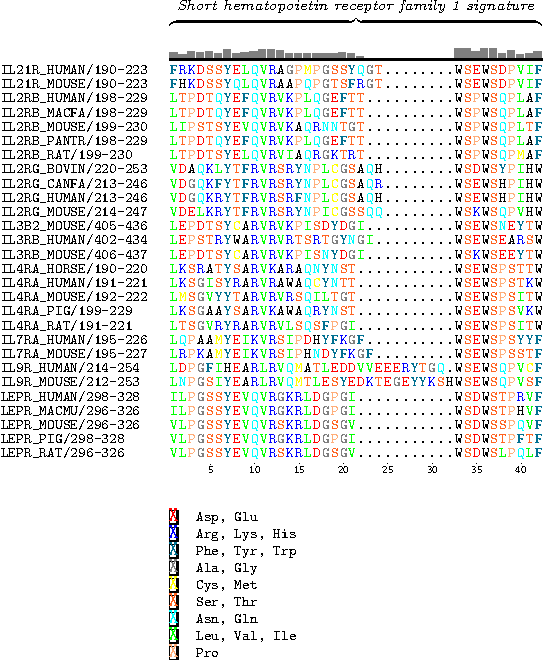
\includegraphics[width=0.80\textwidth]{Body/Images-chap1/hematopo.pdf}
            \caption[Regular grammar describing the short hematopoietin receptor family 1 signature]{
            Regular grammar describing the short hematopoietin receptor family 1 signature~\cite{hofmann1999prosite}.
            These proteins are mostly receptors for interleukin
            cytokines.  They are selectively expressed in lymphoid
            tissues and are typically membrane--bound~\cite{parrish-novak2000interleukin}.  The
            region shown in the figure is characterized by the
            regular expression
            \texttt{[LIVF].........[LIV][RK].(9,20)WS.WS....[FYW]}.
            This motif is required for
            proper protein folding, efficient intracellular transport, and cell--surface receptor
            binding.  The motif is relatively sensitive for the
            receptor family; however, it misses the rodent thymic stromal lymphopoietin protein
            receptors, which are in the same family.  Furthermore,
            the motif is not as specific as it could be --- as shown
            above, the motif matches five receptors for the leptin
            obesity factor, which are not in the same family.
            Notice that the bar at the top shows the degree of
            conservation at each position; the amino acids are
            colored to reflect their physiochemical properties; and,
            the bracketed expressions, such as \texttt{[LIV]}, tend
            to group together amino acids with similar physiochemical properties.
            }
            \label{fig:hemato}
            \end{figure}

Because it is a more compact representation, regular grammars are
usually recorded in regular expression form.  In contrast, more
complex grammars cannot be represented as a simple series of
characters and symbols.  This ease with which they can be
communicated has been one of the factors promoting the widespread
use of regular expressions --- it would be inconvenient to discover
a new protein motif and not be able to record the motif in an easily
interpretable form for publication.

The regular expression formalisms presented here, such as the
bracketed expression and the wild--card, are not exhaustive.  There
are many more terms that increase the richness of regular
expressions, such as the Kleene star, ``\texttt{*}'', which means
``zero or more of the preceding expression'' and the ``\texttt{+}''
symbol, which means ``one or more of the preceding expression.'' For
an exhaustive treatment of regular expressions, the reader is
referred is referred to publications
by~\citet{sipser1997introduction} and~\citet{friedl1997mastering}.

\subsubsection*{Matching regular grammars and regular expressions}

Thus far, I have described how regular expressions be used
to model a set of motif instances.  However, a very common task is
to then use a regular expression to look through new, longer
sequences for ``matches,'' i.e.\ subsequences of a given sequence
that are derivations of the grammar that the regular expression
encodes.  For example, consider the following regular expression:
\texttt{A[KR].Q[LV]C}.  We would like to know if there are any
derivations of this grammar within the sequence shown below.
\begin{equation}\label{eqn:randseq}
    \texttt{FLGARRQLCVVFKLAAKFQVCSKAKWQLCVFPAVFGKV}
\end{equation}
A simpleminded approach to this problem is to start with a beginning
of the sequence, at letter \texttt{F}, and ask whether or not a
derivation of the grammar could start that position.  Obviously, any
derivation of the grammar must begin with an \texttt{A}, so the
answer is ``no.''  Moving on to the first \texttt{A} in the
sequence, we see that it is followed by a \texttt{K}, which is
allowed by the grammar, and that the \texttt{K} can be followed by
any character, etc. Following this procedure reveals three matches
of the regular expression in the sequence, which are underlined
below.
\begin{equation}\label{eqn:randseq2}
    \texttt{FLG\uline{ARRQLC}VVFKLA\uline{AKFQVC}SK\uline{AKWQLC}VFPAVFGKV}
\end{equation}

In general, algorithms designed to match regular expressions against
sequences or other kinds of text use an approach that is, at its
core, the same as the simpleminded approach above.  One such
algorithm and piece of software is described in
Section~\vref{section:biogrep}.


\subsection*{Position weight matrices}\label{section:pwms}
\subsubsection*{Building position weight matrices}

    Despite their utility, regular grammars and regular expressions
    are not suitable for modeling all kinds of motifs.  As I showed
    earlier, regular grammars cannot describe long--range, nested,
    or crossing dependencies between characters.  However, there are
    also motifs where these dependencies do not exist and yet regular
    expressions are not accurate models.

    Consider the collection
    sequences shown in Figure~\vref{fig:yeast}.  This collection
    comprises numerous 3' splice sites from the fission yeast \emph{Schizosaccharomyces
    pombe}.  Each sequence is seven nucleotides in length and
    straddles the intron/exon boundary in a gene.  After
    transcription, these sites will form a ``branch point''
    allowing the introns to be excised from the pre--RNA to form the
    mature mRNA\@.

    Notice that to sensitively describe these sequences using a
    regular expression, we would use
    \texttt{[ATGC][ATGC][CT]T[ATG]A[CT]}.  This motif will match all
    of the instances, but it could also match many more: based on
    the number of bracketed expressions, this regular expression
    would match 192 unique sequences.

    Notice too that each column of the aligned instances shown
    in Figure~\ref{fig:yeast} has a particular ``preference'' for
    one kind nucleotide.  For example, all but 10 of the sequences
    have a thymine at the last position.  But, in the motif
    \texttt{[ATGC][ATGC][CT]T[ATG]A[CT]}, either cytosine or thymine
    is allowed in the last position, without any
    preference.  Obviously, this regular expression would be more
    specific if we labeled the last bracketed expression with these
    preferences, i.e. ``either cytosine or thymine, but with a
    seven--fold preference for the thymine.''


            \begin{sidewaysfigure}[ptb]
            \centering
            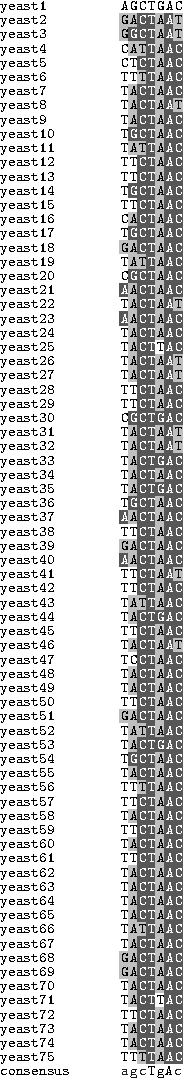
\includegraphics[angle=90]{Body/Images-chap1/yeast.pdf}
            \caption[Yeast 3' splice sites]{Yeast 3' splice sites.  The figure shows the 3'
             splice junction of 75 introns from the fission yeast \emph{Schizosaccharomyces pombe}.
             The coloring of the sequences is used to show the
             degree of conservation.  Notice that certain columns,
             such as the final column, have strong preferences for
             certain nucleotides.  The final column has a strong
             preference for cytosine; however, thymine is allowed
             occasionally.  The consensus sequence at the bottom
             shows the most common nucleotide at each position.  If
             the nucleotide is not perfectly conserved it is shown in
             lowercase.  This kind of motif is poorly modeled using
             regular grammars.  Instead, position weight matrices
             preserve much of the ``preference information.''
            }
            \label{fig:yeast}
            \end{sidewaysfigure}

    Incorporating such preferences into the grammatical framework
    requires only minor changes.  Recall from the definition on
    page~\pageref{gramDefs} that a grammar is
    regular (or right--linear or type--3) if each production in $P$ is of the form
    $A\rightarrow \texttt{x}B$, where $A$ and $B$ are in  $N$
    and $\texttt{x}$ is any string in $\Sigma*$.  A similar set
    of restrictions defines a position weight matrix, which is
    a grammar in which each production in $P$ is of the form
    $A\xrightarrow{p_i} \texttt{x}B$, where $A$ and $B$ are in  $N$
    and $\texttt{x}$ is any \textbf{character} in $\Sigma$,
    and $p_i$ is the probability of production $i$.  As well,
    $\sum_i p_1$ must equal one for all of the productions on which
    $A$ is on the left side.  In loose terms, the position weight
    matrix, or PWM, can be thought of as a probabilistic regular
    expression.  Using this new structure, the regular expression
    \texttt{[ATGC][ATGC][CT]T[ATG]A[CT]} can be written as a PWM
    grammar,
\begin{equation}\label{eqn:pwmGrammar}
    G = (\{S, \alpha, \beta, \gamma, \delta, \epsilon, \zeta, \eta\},\{\texttt{A}, \texttt{T},\texttt{G},\texttt{C}\},P,S),
\end{equation}
where $P$ is the set of productions below.
\begin{align}\label{eqn:pwmProduction}
    P =
    \begin{cases}
    S \rightarrow \alpha \\
    \alpha \xrightarrow{0.067} \texttt{A}\beta \\
    \alpha \xrightarrow{0.773} \texttt{T}\beta \\
    \alpha \xrightarrow{0.093} \texttt{G}\beta \\
    \alpha \xrightarrow{0.067} \texttt{C}\beta \\
    \beta \xrightarrow{0.627} \texttt{A}\gamma \\
    \beta \xrightarrow{0.240} \texttt{T}\gamma \\
    \beta \xrightarrow{0.120} \texttt{G}\gamma \\
    \beta \xrightarrow{0.013} \texttt{C}\gamma \\
    \gamma \xrightarrow{0.120} \texttt{T}\delta \\
    \gamma \xrightarrow{0.880} \texttt{C}\delta \\
    \delta \xrightarrow{1.000} \texttt{T}\epsilon \\
    \epsilon \xrightarrow{0.893} \texttt{A}\zeta \\
    \epsilon \xrightarrow{0.027} \texttt{T}\zeta \\
    \epsilon \xrightarrow{0.080} \texttt{G}\zeta \\
    \zeta \xrightarrow{1.000} \texttt{A}\eta \\
    \eta \xrightarrow{0.133} \texttt{T} \\
    \eta \xrightarrow{0.867} \texttt{C}
    \end{cases}
\end{align}
    Equation~\ref{eqn:hairpinProduction} can be represented much
    more compactly as a frequency matrix
    \begin{equation}\label{eqn:freq}
    f=
        \begin{pmatrix}
0.067 & 0.627 & 0.000 & 0.000 & 0.893 & 1.000 & 0.000 \\
0.773 & 0.240 & 0.120 & 1.000 & 0.027 & 0.000 & 0.133 \\
0.093 & 0.120 & 0.000 & 0.000 & 0.080 & 0.000 & 0.000 \\
0.067 & 0.013 & 0.880 & 0.000 & 0.000 & 0.000 & 0.867
        \end{pmatrix}
    \end{equation}
    in which each row corresponds to a single character in
    $\Sigma$ and each column corresponds to a single non--terminal
    character in  $N$ (where $\Sigma$ is disjoint from $N$, as
    usual).  So, in Equation~\ref{eqn:freq}, the rows correspond to
    \texttt{A}, \texttt{T}, \texttt{G}, and \texttt{C}; and the columns
    correspond to $\alpha$, $\beta$, $\gamma$, $\delta$, $\epsilon$, $\zeta$, and
    $\eta$, where $S$ was omitted.

    Notice that a derivation of the grammar in Equation~\vref{eqn:pwmGrammar}
    is necessarily also a derivation of the regular grammar
    \texttt{[ATGC][ATGC][CT]T[ATG]A[CT]}, and vice versa.  As such, the two grammars
    describe the same language, or the set of all derivations.  But,
    because the productions of Equation~\ref{eqn:pwmGrammar} are
    weighted by probability, certain derivations are more probable
    than others.  The degree to which one derivation of the grammar
    is more probable than another is characterized by the
    derivation's log--odds score.  To compute the log--odds score,
    first requires a log--odds matrix, $\Theta$, where
\begin{equation}\label{eqn:theta}
    \Theta_{ij} = \log_2 \left(\frac{f_{ij}}{q_j}\right).
\end{equation}

    The calculation of the frequency and log--odds matrices for the
    3' yeast splice sites is shown in Table~\ref{table:pwm}.  Here,
    $\Theta$ is given by
    \begin{equation}\label{eqn: theta2}
    \Theta =
        \begin{pmatrix}
-1.907 & 1.326 & \varnothing & \varnothing & 1.837 & 2.000 & \varnothing \\
1.629 & -0.059 & -1.059 & 2.000 & -3.229 & \varnothing & -0.907 \\
-1.421 & -1.059 & \varnothing & \varnothing & -1.644 & \varnothing & \varnothing \\
-1.907 & -4.229 & 1.816 & \varnothing & \varnothing &
\varnothing & 1.794
        \end{pmatrix},
    \end{equation}
    where $\varnothing$ is used to indicate values that are
    undefined because $f_{ij}=0$ and $\log_2 0$ is undefined.
    Given
    the log--odds matrix form of a PWM, the score of any derivation
    of the PWM is computed merely by looking up values in $\Theta$.
    Consider the sequence \texttt{AGCTGAC}, which is both a
    derivation of the grammar shown in Equation~\vref{eqn:pwmGrammar}
    and the first of the sequences shown in Figure~\vref{fig:yeast}.
    The log--odds score for this sequence is
    \begin{equation}\label{eqn:score}
        \begin{split}
          \text{score} &= \Theta_{0,0} + \Theta_{2,1}+ \Theta_{3,2}
                    + \Theta_{1,3}+ \Theta_{2,4}+ \Theta_{0,5}+ \Theta_{3,6}\\
            =& -1.907 -0.059 +1.816 +2.000 -1.644 +2.000 +1.794\\
            =& 4.000.
        \end{split}
    \end{equation}
    Notice that the score for a sequence that is not a derivation of
    the grammar is undefined, or, effectively $-\infty$.
    Table~\vref{table:pwm} shows the calculation of the frequency
    matrix, log--odds matrix, and the scoring of example sequences
    for this PWM\@.  Also, a small program for calculating a
    PWM from a set of sequences is provided in
    Section~\vref{section:pwmCode} of the Appendix.


        \newcolumntype{H}{>{\columncolor[gray]{0.8}}c}

\begin{table}[ptbh]
    \caption[The construction of a position weight matrix]{
        The construction of a position weight matrix from
        the collection of sequences shown in
        Figure~\vref{fig:yeast}.  Part A) shows the number of
        nucleotides of each type that occur in each of the seven
        positions of the aligned sequences.  For example, in the
        first position, there are 58 thymines.  Part B) shows the
        frequency matrix $f$, where each $f_{ij}=(c_{ij}/\sum_j
        c_{ij})$.  Part C) shows the log--odds matrix $\Theta$,
        where each $\Theta_{ij} =  \log_2 (f_{ij}/q_j)$
        and $q$ is the vector of background frequencies for the
        nucleotides.  Part D) shows the scoring of three different
        sequences.  To compute the score for a sequence, the
        corresponding nucleotide at each column is looked up in
        $\Theta$ and the columns are summed together.
        }
            \label{table:pwm}
                    \centering \scriptsize
            \begin{tabular}{r|HcHcHcH} %\hline\hline
\multicolumn{8}{l}{} \\
\multicolumn{8}{l}{A) Count  Matrix ($c_{ij}$):} \\
\multicolumn{8}{l}{} \\
A & 5 & 47 & 0 & 0 & 67 & 75 & 0 \\
T & 58 & 18 & 9 & 75 & 2 & 0 & 10 \\
G & 7 & 9 & 0 & 0 & 6 & 0 & 0 \\
C & 5 & 1 & 66 & 0 & 0 & 0 & 65 \\
  \multicolumn{4}{c}{ }& $\Downarrow$\\
\multicolumn{8}{l}{B) Frequency  Matrix ($f_{ij}$):} \\
\multicolumn{8}{l}{} \\
A & 0.067 & 0.627 & 0.000 & 0.000 & 0.893 & 1.000 & 0.000 \\
T & 0.773 & 0.240 & 0.120 & 1.000 & 0.027 & 0.000 & 0.133 \\
G & 0.093 & 0.120 & 0.000 & 0.000 & 0.080 & 0.000 & 0.000 \\
C & 0.067 & 0.013 & 0.880 & 0.000 & 0.000 & 0.000 & 0.867 \\
  \multicolumn{4}{c}{ }& $\Downarrow$\\
\multicolumn{8}{l}{C) Log--odds  Matrix ($\Theta_{ij}$):} \\
\multicolumn{8}{l}{} \\
A & -1.907 & 1.326 & $\varnothing$ & $\varnothing$ & 1.837 & 2.000 & $\varnothing$ \\
T & 1.629 & -0.059 & -1.059 & 2.000 & -3.229 & $\varnothing$ & -0.907 \\
G & -1.421 & -1.059 & $\varnothing$ & $\varnothing$ & -1.644 & $\varnothing$ & $\varnothing$ \\
C & -1.907 & -4.229 & 1.816 & $\varnothing$ & $\varnothing$ & $\varnothing$ & 1.794 \\
  \multicolumn{4}{c}{ }& $\Downarrow$\\
\multicolumn{8}{l}{D) Example sequence scoring:} \\
\multicolumn{8}{l}{} \\
query1 & T & A & C & T & T & A & C\\
$\Sigma$ & 1.629  & 1.326 & 1.816 & 2.000 & -3.229 & 2.000 & 1.794\\
  \multicolumn{4}{c}{ }& $= 7.335$\\
query2 & T & T & C & T & A & A & C \\
$\Sigma$ & 1.629  & -0.059 & 1.816 & 2.000 & 1.837 & 2.000 & 1.794\\
  \multicolumn{4}{c}{ }& $= 11.017$\\
query3 & G & T & A & T & A & A & T \\
$\Sigma$ & -1.421  & -0.059 & $\varnothing$ \\
  \multicolumn{4}{c}{ }& $= \varnothing$\\
%\hline\hline
\end{tabular}
\end{table}


    The ``strength'' of a PWM motif is measured by a quantity called
    its entropy.  The motif entropy is the sum of the entropies of
    each column, or position in the motif.
    This entropy of a given column in a PWM is a measure of the
    disorder, or the randomness of the distribution of letters.  The
    column entropy is measured in bits and is given by
        \begin{equation}\label{eqn:pwmh}
            h_i = -\sum_{j} f_{ij}\log_2 f_{ij}
        \end{equation}
    where, $f_{ij}$ is the frequency matrix as shown in
    Figure~\vref{table:pwm}.  The entropy of the whole motif
    is just the sum of the entropies of the columns:
        \begin{equation}\label{eqn:pwmH}
            H = -\sum_{i}\sum_{j} f_{ij}\log_2 f_{ij}.
        \end{equation}

    Typically, the entropy is measured
    relative to the background entropy.  As above, the background
    entropy of a single column is
        \begin{equation}\label{eqn:pwmbgh}
            h_i^\circ = -\sum_{j} q_{j}\log_2 q_{j}
        \end{equation}
    where, $q_{j}$ is the \emph{a priori}, background frequency of
    the letter denoted by index $j$.  In the case of identically
    distributed nucleotides, each $q_j$ is $0.25$; i.e.\ $q_A=0.25$,
    $q_C=0.25$, $q_T=0.25$, and $q_G=0.25$.  The background entropy
    of the entire motif is
        \begin{equation}\label{eqn:pwmbgH}
            H^{\circ} = -\sum_{i}\sum_{j} q_j\log_2 q_j.
        \end{equation}

    The difference between the background entropy and the motif
    entropy is referred to as the information content, $I$, of the PWM\@.
    Using Equations~\ref{eqn:pwmh}--~\ref{eqn:pwmbgH} above, the
    information content can be calculated as
        \begin{equation}\label{eqn:pwmI}
            \begin{split}
              I &=  H^{\circ}-H\\
                &= -\sum_{i}\sum_{j} q_j\log_2 q_j - \left(-\sum_{i}\sum_{j}f_{ij}\log_2 f_{ij}\right)\\
                &= \sum_{i}\sum_{j}f_{ij}\log_2
                \left(\frac{f_{ij}}{q_j}\right).
            \end{split}
        \end{equation}
    Notice that the information content of the motif is minimized
    when the nucleotide distribution for each column is exactly the
    background distribution of nucleotides.  That is, when $f_{ij}=q_j$
    for all $i$, the $\log_2(f_{ij}/q_j)$ terms are zero.
    This makes sense intuitively: if the PWM describes the
    background distribution, the motif can obviously not be
    distinguished from the background and therefore contains no
    information.  In this same case, the entropy of the motif is
    maximized and is equal to the background entropy.

    PWMs are commonly represented by two varieties of schematics:
    pictograms and sequence logos.  An example of each of these is
    shown in Figure~\vref{fig:yeastLogo}.
    A pictogram is essentially a visualization of the frequency
    matrix representing a PWM, whe, whereas  A sequence logo is a pictogram
    that is scaled to reflect the information content at each
    position in the PWM\@.

            \begin{figure}[ptb]
        A) Pictogram of the PWM in Table~\vref{table:pwm}
            \begin{center}
            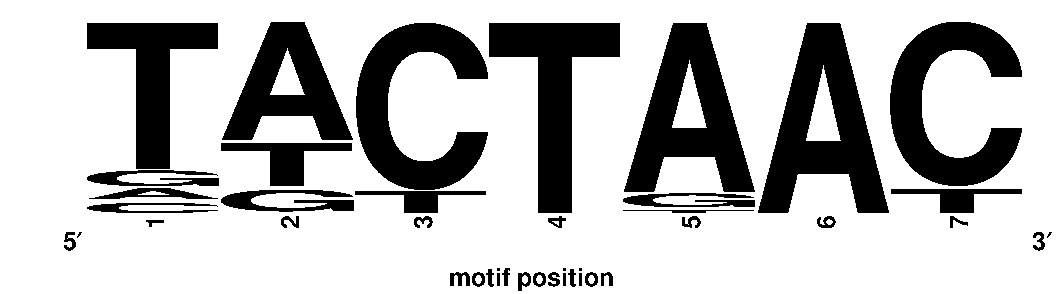
\includegraphics[width=\textwidth]{Body/Images-chap1/yeast-logo2.pdf}
            \end{center}
        \bigskip
            B) Logo of the PWM in Table~\vref{table:pwm}
            \begin{center}
        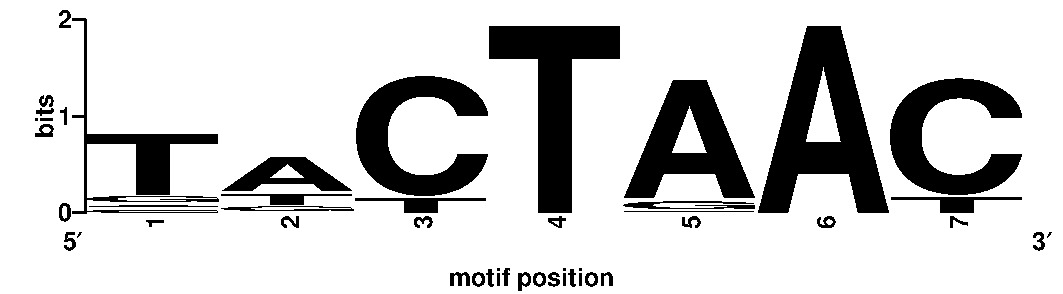
\includegraphics[width=\textwidth]{Body/Images-chap1/yeast-logo1.pdf}
            \end{center}
            \caption[Yeast 3' splice site pictogram and logo]{
            Yeast 3' splice site pictogram and logo. Part A) shows
            the
            PWM in Table~\vref{table:pwm} represented as a
            pictogram.  At each position in the motif, the height of
            the nucleotides is scaled in proportion to their
            frequency in $f$, with the more frequent nucleotides
            always placed on top.  The pictogram clearly shows that
            positions four and six are perfectly conserved, whereas
            the other positions are distributed between many
            nucleotides.  Part B) shows a sequence logo
            representation of the same PWM.  The sequence logo is a
            pictogram in which the height of each column is scaled
            in proportion to the information content contributed by
            that position to the motif (see
            Equation~\vref{eqn:pwmI}).  Taller columns have a
            nucleotide distribution that deviates strongly from the
            background distribution.  In this sequence logo, the
            background distribution is arbitrarily set to equal
            \emph{a priori} probability of each nucleotide.  As
            such, the maximum information content in any column is
            two bits, which is achieved only in the two perfectly
            conserved positions of the motif.
            }
            \label{fig:yeastLogo}
            \end{figure}

\subsubsection*{Matching position weight matrices}

        Thus far, I have shown how a PWM can be used to model a
        set of motif instances and how a derivation of a PWM
        grammar can be scored.  PWMs can also be used to search in
        new, long sequences for regions of the sequence that appear
        to match the motif.  This is accomplished by ``sliding'' the
        PWM over the length of the sequence to look for subsequences
        that have high log--odds scores.

        Consider searching the sequence \texttt{TAGCTGACTGAC}.  To
        slide the PWM over this sequence is equivalent to evaluating
        the score of each seven nucleotide substring:
        \texttt{TAGCTGA},
        \texttt{AGCTGAC},
        \texttt{GCTGACT},
        \texttt{CTGACTG},
        \texttt{TGACTGA}, and
        \texttt{GACTGAC}.  These are $\varnothing$, 4.0,
         $\varnothing$, $\varnothing$, $\varnothing$, and
         5.871.  That is, there are two matches for the PWM, one
         stronger than the other.  This method can be used to search
         for a PWM in much larger sequences as well.  For example,
         Figure~\ref{fig:pwmHits} (page~\pageref{fig:pwmHits}) shows the distribution of scores
         obtained by searching
            the PWM in Table~\vref{table:pwm} against chromosomes 1--4 of
        the
            \emph{Saccharomyces cerevisiae} genome.


            \begin{figure}[ptb]
            \centering
            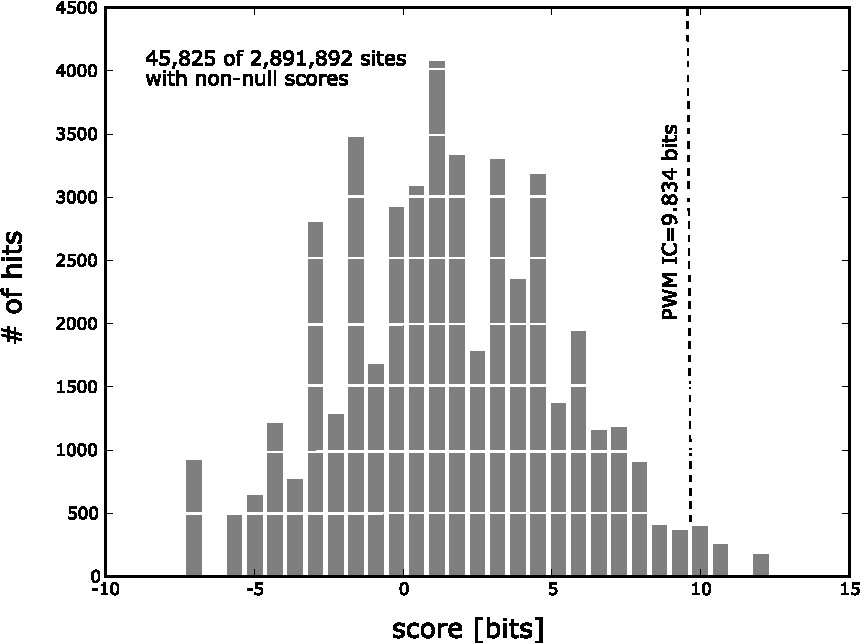
\includegraphics[width=\textwidth]{Body/Images-chap1/pwmHits.pdf}
            \caption[pwmHits]{Distribution of log--odds scores obtained by searching
            the PWM in Table~\vref{table:pwm} against chromosomes 1--4 of
            \emph{Saccharomyces cerevisiae}.  Of the nearly 3
            million possible sites, only 46,000 had non--null
            scores.  As the figure shows, the score distribution is
            roughly Gaussian.  The dashed line indicates the
            information content of the PWM\@.  Scores above this
            line are generally considered  strong matches.
            PWMs are more specific than regular grammars, because
            the threshold above which a match is considered ``true''
            can be varied.  In contrast, with a regular grammar is
            either a match or not a match: there is no variable threshold.
        }
            \label{fig:pwmHits}
            \end{figure}



\section{Tools for motif discovery}\label{section:tools}
\subsection*{Introduction}

    In general, the goal of motif discovery is to derive a set of
    grammars that sensitively matches a set of given sequences.
    This is the inverse of many of the examples in the previous
    section.  That is, imagine a case in which you are given a set
    of derivations and then asked what kind of grammar could have
    produced the derivations?  This is what is called grammar
    induction in  the computational linguistics literature and is
    equivalent to guessing the grammar of an unknown language given a few
    sentences in the language.

    In bioinformatics, this task is usually presented in a slightly
    more difficult form.  To illustrate this, consider a
    hypothetical challenge in which a colleague hides derivations of
    the regular grammar \texttt{[KR]QTRP.[RT]K} in a set of
    sequences that consist otherwise of random characters.  You are
    presented with the sequences and asked what grammar was hidden
    therein.
    \begin{equation}\label{eqn:hidden1}
        \begin{split}
          \texttt{AJDFIOASODVIKQTRPXYKIIWEJSJ} \\
          \texttt{JKQTRPCRKXUCIQWEMFIOAKLGS} \\
          \texttt{ADUHFIKACRQTRPXKMSKDAFIOAS}
        \end{split}
    \end{equation}
    Without any prior knowledge, this task is nearly impossible.
    The colleague could have hidden a regular grammar that consisted
    solely of \texttt{S}, which would be undetectable since there are many characters
    that occur in all of the sequences.  Further, he could have hidden ``\texttt{....}'',
    in which case there would be no evidence in the sequences.
    This conundrum is closely related to one of the three tenets
    of motif discovery
    developed in Section~\vref{section:tenents}: the answer to any
    motif discovery question is invariably dependent on at least
    some prior knowledge about what forms a motifs may take.

    Suppose then that the colleague says the motif is at least five
    characters long, is a regular grammar, and all the derivations
    of the grammar look ``pretty similar.''  Given this
    information, a logical approach would be to look for
    subsequences of five characters that look relatively similar and
    occur in all three sequences.  After diligently scanning the
    sequences, you can find two sets of three that seemed to fit
    this description: $\{\texttt{FIOAS}, \texttt{FIOAK},
    \texttt{FIOAS}\}$ and $\{\texttt{KQTRP}, \texttt{KQTRP},
    \texttt{RQTRP}\}$.  Knowing the answer, it is obvious that we
    are on the right track; however, again we are at an impasse.
    It would be easy to write a regular expression describing either
    of these sets.  But, \emph{a priori} it is impossible to tell
    which set may be the correct answer.  The first set has a \texttt{K}
    that is mismatched with a \texttt{S}, whereas the latter set has
    a \texttt{K}--\texttt{R} mismatch.  If these were amino acid
    sequences we could say that lysine, \texttt{K}, is more similar
    to arginine, \texttt{R}, than it is to serine, \texttt{S}.
    Therefore, we might choose the latter set.  This decision is
    related to the remaining two tenets of motif discovery developed
    in Section~\ref{section:tenents}: the answer to any motif
    discovery problem will always depend on a predefined metric of
    similarity and a method for grouping together similar objects.


    In the following sections, I review a number of approaches for
    problems such as the example given above,
    focusing on the two most common classes of
    approach: those that use regular expression motif models and
    those that use PWMs.  All of these approaches, without
    exception, always require some degree of intelligent guidance by
    the user that can be reduced to the three tenets discussed
    above.  In general, motif discovery tools that do not have such
    requirements have made assumptions on the user's behalf.



\subsection*{Teiresias and other regular expression--based
tools}\label{section:teiresias}

    Because they are convenient from both a computational
    perspective and from the perspective of communicating results,
    regular expressions are the most common form of motif model used
    in bioinformatics.  Table~\vref{table:regexMD} shows a list of
    publications introducing motif discovery tools in this class.
    Within the field, these algorithms are commonly referred to as ``motif driven''
    or ``pattern driven''
            algorithms~\cite{brazma1998pattern}.
            At their most basic conceptual level, all of these
            approaches work by first enumerating possible patterns
            and then checking for the patterns in the sequence
            set~\cite{brazma1998pattern}.

            There are three principal characteristics that distinguish between the various
            algorithms shown in Table~\ref{table:regexMD}, which are as
            follows:
            \begin{enumerate}
                \item   The regular expression class complexity.
                \item   The completeness of the returned motif set.  That is, does the algorithm return \emph{all}
                        patterns present in the input sequences?
                \item   The motif \emph{maximality}.  For instance, in the two strings ``\texttt{KYLEJ}'' and ``\texttt{KYLEL}'',
                        the motif ``\texttt{KYLE}'' is maximal, whereas ``\texttt{KYL}'' is not, because we could
                        add an ``\texttt{E}'' without decreasing the number of times it
                        occurs.  In essence, maximality is a proxy
                        for specificity.
            \end{enumerate}

        \begin{table}[ptbh]
    \caption[Motif discovery tools using regular expressions or similar models]{
        Motif discovery tools using regular expressions or similar
        models.  This list is not intended to be exhaustive;
        however, it includes many of the well--known motif discovery
        tools used in bioinformatics.  Early methods tended to use
        consensus strings or simple word counting approaches, i.e.\
        counting the occurrences of ``n--mers'' such as the 4--mer
        \texttt{ATGC}.  Words that are statistically over--represented
        are called motifs.  Later approaches used more complex
        regular expressions, cf.~\citet{rigoutsos1998combinatorial}.
        }
            \label{table:regexMD}
                    \centering
            \begin{tabular}{lcc} \hline\hline
Authors & Year & Citation \\ \hline
\citeauthor{queen1982improvements} & \citeyear{queen1982improvements} & \cite{queen1982improvements} \\
\citeauthor{galas1985rigorous} & \citeyear{galas1985rigorous} & \cite{galas1985rigorous} \\
\citeauthor{mengeritsky1987recognition} & \citeyear{mengeritsky1987recognition} & \cite{mengeritsky1987recognition} \\
\citeauthor{staden1989methods} & \citeyear{staden1989methods} & \cite{staden1989methods} \\
\citeauthor{neuwald1994detecting} & \citeyear{neuwald1994detecting} & \cite{neuwald1994detecting} \\
\citeauthor{jonassen1995finding} & \citeyear{jonassen1995finding} & \cite{jonassen1995finding} \\
\citeauthor{wolferstetter1996identification} & \citeyear{wolferstetter1996identification} & \cite{wolferstetter1996identification} \\
\citeauthor{sagot1997multiple} & \citeyear{sagot1997multiple} & \cite{sagot1997multiple} \\
\citeauthor{rigoutsos1998combinatorial} & \citeyear{rigoutsos1998combinatorial} & \cite{rigoutsos1998combinatorial,floratos1999pattern} \\
\citeauthor{van1998extracting} & \citeyear{van1998extracting} & \cite{van1998extracting,van2000discovering} \\
\citeauthor{jacobs2000computational} & \citeyear{jacobs2000computational} & \cite{jacobs2000computational} \\
\citeauthor{marsan2000algorithms} & \citeyear{marsan2000algorithms} & \cite{marsan2000algorithms} \\
\citeauthor{pevzner2000combinatorial} & \citeyear{pevzner2000combinatorial} & \cite{pevzner2000combinatorial} \\
\citeauthor{bussemaker2000building} & \citeyear{bussemaker2000building} & \cite{bussemaker2000building} \\
\citeauthor{kielbasa2001combining} & \citeyear{kielbasa2001combining} & \cite{kielbasa2001combining} \\
\citeauthor{horton2001tsukuba} & \citeyear{horton2001tsukuba} & \cite{horton2001tsukuba} \\
\citeauthor{keich2002subtle} & \citeyear{keich2002subtle} & \cite{keich2002subtle} \\
\citeauthor{eskin2002finding} & \citeyear{eskin2002finding} & \cite{eskin2002finding} \\
\citeauthor{buhler2002finding} & \citeyear{buhler2002finding} & \cite{buhler2002finding} \\
\citeauthor{sinha2002discovery} & \citeyear{sinha2002discovery} & \cite{sinha2002discovery} \\
\citeauthor{price2003finding} & \citeyear{price2003finding} & \cite{price2003finding} \\
\citeauthor{sinha2003discriminative} & \citeyear{sinha2003discriminative} & \cite{sinha2003discriminative} \\
\citeauthor{danilova2003an} & \citeyear{danilova2003an} & \cite{danilova2003an} \\
\citeauthor{ganesh2003mopac} & \citeyear{ganesh2003mopac} & \cite{ganesh2003mopac} \\
\citeauthor{liang2004cwinnower} & \citeyear{liang2004cwinnower} & \cite{liang2004cwinnower} \\
\citeauthor{fogel2004discovery} & \citeyear{fogel2004discovery} & \cite{fogel2004discovery} \\
\citeauthor{pavesi2004weeder} & \citeyear{pavesi2004weeder} & \cite{pavesi2004weeder} \\
\citeauthor{hernandez2004model} & \citeyear{hernandez2004model} & \cite{hernandez2004model} \\
\citeauthor{markstein2004regulatory} & \citeyear{markstein2004regulatory} & \cite{markstein2004regulatory} \\
\citeauthor{frith2004finding} & \citeyear{frith2004finding} & \cite{frith2004finding} \\
\citeauthor{sumazin2005dwe} & \citeyear{sumazin2005dwe} & \cite{sumazin2005dwe} \\
\hline
\end{tabular}
\end{table}


            The most important of these distinguishing features
            is the complexity of the regular expression class that
            an algorithm returns.  No motif discovery tool can
            search for the ``universe'' of regular expressions.
            Recall from the previous section that ``\texttt{...}''
            and other types of motifs will always be present, and
            therefore such a result is meaningless.  Furthermore,
            enumerating regular expressions is
            NP--complete~\cite{maier1978complexity,garey1979computers},
            meaning that, in general, the runtime of a motif
            discovery tool will increase exponentially with the size
            of the sequence set it is given.  As I showed in the
            previous section, the answer to any motif discovery
            problem will always require some \emph{a priori}
            knowledge of the kinds of motifs that might be found, and
            simply specifying that the grammar is regular is not
            enough.  Accordingly, most motif discovery tools
            restrict themselves to finding a particular subclass of
            regular expressions.
            This motif class determines the form of each
            pattern, $p_i$ that we find.  Below, a few motif classes, commonly
            used in biological sequence analysis,  are enumerated in
            order of increasing complexity~\cite{floratos1999pattern}:

            \begin{itemize}
                \item   $p_i\in\Sigma^{\ast}$:  This is the class
                        of all ``solid'' patterns, for example
                        ``\texttt{KAGTPT}'' and ``\texttt{TAGCGGGAT}''.

                \item   $p_i\in(\Sigma\cup\{.\})^{\ast}$:  This is the
                        class of all patterns that can have ``wildcard''
                        positions, which are denoted by ``.'', for example
                        ``\texttt{K.G.PT}'' and ``\texttt{TA...GGAT}''.
                        The wildcard means that any character from the
                        alphabet will suffice in that position.

                \item   $p_i\in(\Sigma\cup R)^{\ast}$: This
                        is the class of all patterns that can
                        have ``bracketed'' expressions, for
                        example ``\texttt{K[ADG]G[KQ]PT}'' and
                        ``\texttt{TA[GA][TC]GGAT}''.  The bracketed
                        expression ``[\texttt{TC}]'' means that either
                        ``\texttt{T}'' or ``\texttt{C}'' will suffice in
                        that position.  In this notation, $R$ represents
                        the set of characters in the brackets, for example
                        $R=\{\texttt{TC}\}$ or $R=\{\texttt{GA}\}$.

                \item   $p_i\in(\Sigma\cup .)^{\ast}$:  This is the
                        class of ``flexible'' patterns.  For example
                        ``\texttt{K.(1,3)G.(2,5)PT}'', where ``.(2,5)''
                        means that anywhere between two and five wildcards
                        can exist at that position, that is .(2,5)
                        can be any one of $\{..,...,....,......\}$.

            \end{itemize}
            In general, the more complex these patterns are, the more expressive the languages will be that we find.  However,
            with increasing complexity, the computational difficulty of the motif discovery problem increases
            drastically~\cite{maier1978complexity,garey1979computers}.



            Also, for some of these tools, it is possible to
            guarantee the completeness of the set of returned
            patterns.  That is, a particular tool may guarantee that all
            regular expressions meeting particular characteristics are discovered.
            However, this guarantee comes at the price of
            increased time and space complexity.  That is, the set
            of all possible patterns is very large and can take a
            large space to enumerate and a long time to search
            through.  As such, many motif driven algorithms
            use heuristics to limit the space of patterns that are
            searched.

            Here, I will focus on the Teiresias algorithm as a representative
            regular expression--based motif discovery tool.
            Notably, Teiresias is the basis for much of the work in
            this thesis, particularly in Chapters 1 and 2.
            A more detailed description of Teiresias is available elsewhere~\cite{floratos1999pattern,rigoutsos1998combinatorial}.


            Given a set of sequences $S = \{ s_0,s_1,\ldots,s_n\}$,
            and integers $L$, $W$, and $K$, Teiresias finds all
            patterns involving at least $L$ non--wildcard characters
            that occur at least $K$ times and have a fraction of
            non--wildcard characters of at least $L/W$.  This set of
            patterns is called $\mathcal{C}$, where $\mathcal{C}=\{
            p_1,p_2,\ldots,p_m\}$ and each $p_i\in\teirRegEx$.
            This is the set of all regular expressions that begin
            and end with a character, but may have an arbitrary
            number of wild--cards and characters in the middle
            subject to the $L$ and $W$ restriction,
            for example, \texttt{AXG}, \texttt{A.G},
            \texttt{K..R.G}, etc.
            For
            each motif $p_i$ in $\mathcal{C}$, Teiresias returns an
            offset list $\mathscr{L}\paren{p_i}$ that specifies each
            sequence--position combination where the motif occurs
            (cf.\ Figure~\vref{fig:teiresias output}).

            The support of a motif is equal to
            the number of its occurrences (or, equivalently, ``instances'' or ``embeddings''),
            $\vert \mathscr{L}(p) \vert$.
            Essentially,
            $L$ defines the minimum size of patterns in which we are
            interested, and $L/W$ defines the minimum specificity
            (the fewer wildcards, the more specific a motif).
            The four distinguishing characteristics of the Teiresias algorithm are as follows:
            \begin{enumerate}
                \item   All \emph{maximal} patterns are reported (see below for a definition of ``maximal'').
                \item   Only the maximal patterns are reported.
                \item   Running time depends only on the number of patterns present in
                        the data, that is it is \emph{output sensitive}.
                \item   Patterns can be arbitrarily long.
            \end{enumerate}
            The most important characteristic of Teiresias is that it returns the \emph{complete} set of maximal patterns.
            And, because of the manner in which these patterns are handled internally by Teiresias, the algorithm runs
            very quickly.

    In the Teiresias parlance, a maximal motif is a regular expression which has the following properties:
        \begin{enumerate}
        \item   The motif cannot be made more specific
            without producing a motif with
            fewer embeddings (i.e., without
            $\vert \mathscr{L}(p) \vert$
            decreasing); and

        \item   The motif is not missing any instances,
            i.e.\ $\mathscr{L}(p)$ includes the locations
            of all instances of the motif.

        \end{enumerate}
    These two criteria can be summarized qualitatively by stating that a maximal
    motif is not ``missing'' any locations and is as wide as possible, and
    thus it is as specific and sensitive as possible.  Here,
    ``specific'' has a particular meaning: a pattern $p_i$ is more
    specific than $p_j$ if $p_j$ can be transformed into $p_i$ by
    substituting one or more wild--cards for a character, or by
    appending wild--cards and characters to either side of $p_j$.
    For example, \texttt{CH.MEN..N} is less specific than all of the
    following regular expressions: \texttt{CHEMEN..N},
    \texttt{CH.MEN..NE.R},
    and \texttt{CH.MEN.IN}.
    Necessarily, if a pattern $p_i$ is more specific than a pattern $p_j$, then
    \begin{equation}\label{eqn:support}
        \vert \mathscr{L}(p_i) \vert \leq
        \vert \mathscr{L}(p_j) \vert .
    \end{equation}

    Teiresias works in two phases: scanning and convolution.
    During the scanning phase, Teiresias enumerates
    all ``elementary motifs'' with exactly $L$ characters and at most $W-L$
    wild--cards (see Figure~\vref{fig:teiresiasExample}).
    Elementary motifs are short regular expressions that can be
    stitched together to form longer regular expressions that are
    more specific, using the definition of specificity above.  For
    example, as shown in Figure~\ref{fig:teiresiasExample}, the
    sequences
    \begin{equation*}
        \begin{split}
          \texttt{KDWVQKRK} \\
          \texttt{CWCQKRK} \\
          \texttt{WDQKRKNP}
        \end{split}
    \end{equation*}
    have five motifs with 1) exactly $L=3$ characters, 2) no more than
    $W-L$ wild--cards for every window of $L=3$ characters,
    and that 3) occur at least three times:
    \texttt{W.QK}, \texttt{QKR}, \texttt{QK.K}, \texttt{KRK},
    and \texttt{Q.RK}.  These are the elementary motifs.

           \begin{figure}[ptb]
            \centering
\begin{verbatim}
                           >seq 0
                           KDWVQKRK
                           >seq 1
                           CWCQKRK
                           >seq 2
                           WDQKRKNP
\end{verbatim}

            $\Downarrow$\\
    Teiresias\\
    $L/W/K = 3/4/3$ \\
            $\Downarrow$\\

            Elementary motifs: \\

            \begin{tabular}{lccccc} \hline\hline
            motifs $\rightarrow$ & \texttt{W.QK~~} & \texttt{~~QKR}& \texttt{~~QK.K}& \texttt{~~~KRK}&
            \texttt{~Q.RK}\\ \hline
            \multirow{2}{*}{offset \#0} &
            \texttt{KD\textbf{W}V\textbf{QK}RK~~} &
            \texttt{KDWV\textbf{QKR}K~~} &
            \texttt{KDWV\textbf{QK}R\textbf{K}~~} &
            \texttt{KDWVQ\textbf{KRK}~~} &
            \texttt{KDWV\textbf{Q}K\textbf{RK}~~} \\
            & (0,2)
            & (0,4)
            & (0,4)
            & (0,5)
            & (0,4)\\ \hline
            \multirow{2}{*}{offset \#1} &
            \texttt{~C\textbf{W}C\textbf{QK}RK~~} &
            \texttt{~CWC\textbf{QKR}K~~} &
            \texttt{~CWC\textbf{QK}R\textbf{K}~~} &
            \texttt{~CWCQ\textbf{KRK}~~} &
            \texttt{~CWC\textbf{Q}K\textbf{RK}~~} \\
            & (1,1)
            & (1,3)
            & (1,3)
            & (1,4)
            & (1,3) \\ \hline
            \multirow{2}{*}{offset \#2} &
            \texttt{~~\textbf{W}D\textbf{QK}RKNP} &
            \texttt{~~WD\textbf{QKR}KNP} &
            \texttt{~~WD\textbf{QK}R\textbf{K}NP} &
            \texttt{~~WDQ\textbf{KRK}NP} &
            \texttt{~~WD\textbf{Q}K\textbf{RK}NP} \\
            & (2,0)
            & (2,2)
            & (2,2)
            & (2,3)
            & (2,2) \\ \hline\hline
            \end{tabular}
            \caption[Scanning phase of Teiresias]{
            Scanning phase of Teiresias.  During the scanning phase, Teiresias enumerates
            all elementary motifs with exactly $L$ characters and at most $W-L$ wild--cards.
            Using the input sequences above, Teiresias finds five such elementary motifs
            as shown in the table: \texttt{F.AS}, \texttt{AST}, \texttt{AS.S}, \texttt{STS}, and
            \texttt{A.TS}.  The offset list for each of these is shown in the table.
            In the next phase of the algorithm, these elementary motifs are convolved
            together to form the final, maximal motifs.}
            \label{fig:teiresiasExample}
            \end{figure}

            In the convolution phase, the elementary motifs are
            stitched together to see if more specific motifs can be
            found.  The process of convolution is defined as
            follows:
    \begin{equation}\label{eqn:convolution}
    \begin{split}
        p_k &= p_i \oplus p_j\\
        & =
        \begin{cases}
        p_k p_i' & \text{if $\suffix_L(p_i)=\prefix_L(p_j)$,}\\
        \varnothing & \text{otherwise.}
        \end{cases}
    \end{split}
    \end{equation}
    In the equation above $\prefix_L(p_i)$ is  the sub--pattern
    at the beginning of
    $p_i$ with exactly $(L-1)$ characters.  Similarly, $\suffix_L(p_i)$ is  the sub--pattern
    at the end of
    $p_i$ with exactly $(L-1)$ characters.  For example:
    \begin{equation}\label{eqn:prefixsuffix}
        \begin{split}
          \prefix_3(\texttt{W.QK}) & = \texttt{W.Q} \\
          \suffix_3(\texttt{W.QK}) & = \texttt{QK} \\
          \prefix_3(\texttt{QKR}) & = \texttt{QK} \\
          \suffix_3(\texttt{QKR}) & = \texttt{KR}~.
        \end{split}
    \end{equation}
    To illustrate this, consider the following examples:
    \begin{equation*}
    \begin{split}
        \texttt{DF.A.T}\oplus\texttt{A.TSE}&=\texttt{DF.A.TE}\\
        \texttt{L.XF.A.MM}\oplus\texttt{A.MSE}&=\texttt{L.XF.A.MME}\\
        \texttt{WX.N.N}\oplus\texttt{N.PSE}&=\varnothing.
    \end{split}
    \end{equation*}

    If two motifs can be convolved --- i.e.\ $p_i \oplus
    p_j\neq\varnothing$ --- then the offsets of the new,
    longer regular expression, $p_k$ are given by
    \begin{equation}\label{eqn:offsetSize}
        \mathscr{L}(p_k) = \left\{(x,y) \in \mathscr{L}(p_i) \vert
            ~\exists(x,z)\in\mathscr{L}(p_j) \text{~such that~}
            z-y=\mathscr{W}(p)-\mathscr{W}(\suffix_L(p))\right\}.
    \end{equation}
    If $\vert \mathscr{L}(p_k) \vert < K$ then the motif does not
    have sufficient support and is discarded.  Conversely,
    if $\vert \mathscr{L}(p_k) \vert = \vert \mathscr{L}(p_i) \vert$
    then $p_i$ is not a maximal motif.  Or if $\vert \mathscr{L}(p_k) \vert = \vert \mathscr{L}(p_j) \vert$
    then $p_j$ is not a maximal motif.  But, if
    \begin{equation}\label{eqn:conv4}
            \vert p_i \oplus p_j \vert < K\text{~}\forall\text{~}j,
    \end{equation}
    then $p_i$ is maximal.


    Obviously, by convolving each elementary motif with every other
    elementary motif,
    i.e. by repeating $p_k = p_i \oplus p_j$ for all $i$ and $j$,
    the maximal motifs can be discovered.
    Teiresias uses an intelligent method of sorting the elementary
    motifs that does not require doing the all--by--all comparison
    and yet still guarantees that all the maximal motifs are
    discovered.  The set of these maximal motifs are then returned
    to the user as in Figure~\vref{fig:teiresias output}.


            \begin{figure}[ptb]
\begin{verbatim}
    >sequence 0
    MSKNIVLLPGDHVGPEVVAEAVKVLEAVSSAIGVKFNFSKHLIGGASIDAYGVPLSDEALEAAKK
    >sequence 1
    MSKQILVLPGDGIGPEIMAEAVKVLELANDRFQLGFELAEDVIGGAAIDKHGVP
    >sequence 2
    MKFLILLFNILCLFPVLAADNHGVGPQGASGVDPITFDINSNQTGPAFLT
\end{verbatim}

            \centering
            $\Downarrow$\\
    Teiresias:\\
    $L/W/K = 5/8/2$ \\
            $\Downarrow$\\

            Final motifs:\\

            \begin{tabular}{cccc} \hline\hline
            % after \\ : \hline or \cline{col1-col2} \cline{col3-col4} ...
            motif & \multicolumn{2}{c}{location (seq,pos)} \\ \hline
            \ttfamily GPE..AEAVKVLE & (0,13) & (1,13) \\
            \ttfamily IGGA.ID..GVP & (0,42) & (1,42) \\
            \ttfamily MSK.I..LPGD..GPE & (0,0) & (1,0) \\
            \ttfamily A.D.HGV & (1,46) & (2,17)\\ \hline\hline
            \end{tabular}
            \caption[Pattern discovery with Teiresias]{Pattern discovery with Teiresias.  Here we have three protein
            sequences and we use Teiresias to find all patterns involving at least $L=5$ non--wildcard characters that occur
            at least $K=2$ times and have a fraction of non--wildcard characters of at least $L/W=5/8$.  These are called $5/8/2$
            patterns and there are three such patterns in this set of sequences.  Along with each motif is an offset list $\mathscr{L}\paren{p_i}$
            that specifies each sequence--position combination where the motif occurs.  For motif $p_3=$``\texttt{A.D.HGV}'' the
            associated offset list is $\mathscr{L}\paren{p_3}=\{(1,46),(2,17)\}$, indicating that this motif occurs twice: once in sequence
            1 at position 46 and once in sequence 2 at position 17.}
            \label{fig:teiresias output}
            \end{figure}

            The broad applicability of Teiresias has been shown in
            numerous studies.  In particular, the algorithm has
            been very successful in multiple sequence
            alignment~\cite{parida1998musca}, motif dictionary
            building~\cite{rigoutsos1999dictionary}, and gene
            finding in microbial
            genomes.  In the work
            here, we will expand upon these studies in our
            application of the Teiresias motif discovery
            engine to practical problems of interest to the biology
            community, cf.\ Chapter 2.

 \begin{comment}

 Sequence driven
            algorithms align a set of strings, which are presumed to
            be similar, producing a ``consensus
            sequence''~\cite{gusfield1997algorithms}.   This
            consensus sequence is, in essence, an average of the
            input sequences and is used to capture patterns in the
            input sequences (cf.\
            Figure~\vref{fig:consensusSequence})\cite{neville1997enumerating}.
            The most well--known sequence driven syntactic motif
            discovery algorithm is
            BLOCKS~\cite{henikoff1991automated}, others include
            EMOTIF~\cite{neville1997enumerating} and algorithms by
            Martinez~\cite{martinez1988flexible}, Smith
            \etal~\cite{smith1990automatic}, Vingron
            \etal~\cite{vingron1991motif},
            Shinohara~\cite{shinohara1982poly},
            Nix~\cite{nix1984editing},
            Roytberg~\cite{roytberg1992search},
            Schuler~\cite{schuler1991workbench},
            Brodsky~\cite{brodsky1992mathematical}, and
            Clift~\cite{clift1986sequence}. Sequence driven
            syntactic motif discovery algorithms, because they allow
            for insertions and deletions, are capable of finding
            relatively complex flexible
            patterns~\cite{floratos1999pattern}.  Also, by using
            common sequence alignment tools, which use heuristical
            short--cuts, they typically have low run--time costs.
            However, because a number of input sequences are
            required to produce a single consensus sequence, these
            motif discovery algorithms typically are not guaranteed
            to find \emph{all} the patterns.  Additionally, sequence
            driven algorithms are not guaranteed to be maximal.  As
            such, these algorithms are best--suited to situations in
            which the input sequences are known to be globally
            similar and finding all of the patterns is not
            important.
 \end{comment}

\subsection*{Gibbs sampler and other position weight matrix--based tools}

As described in Section~\vref{section:pwms}, PWMs can be much more
specific than regular expressions for modeling a set of motif
instances.  But, this motif model also presents some unique
difficulties.  Recall that, as described in
Section~\vref{section:teiresias}, most regular expression--based
motif discovery tools are ``pattern driven'' in the sense that, at
some level, they rely on enumerating possible regular expressions
and then determining which of those has a significant support within
a given set of sequences.  A similar approach does not work for PWMs
because the set of production probabilities (see
Equation~\vref{eqn:pwmProduction}), or equivalently the target
frequencies in the $f$ matrix (see Equation~\vref{eqn:freq}), are
sampled from a continuous distribution.  Therefore, the set of
possible PWMs cannot be enumerated \emph{a priori} because they are
effectively infinite.

Most motif discovery tools that use PWM models skirt this issue by
taking a more focused approach.  Instead of returning a large set of
motifs, as is common for regular expression--based tools such as
Teiresias, PWM--based tools usually return either one or a small set
of motifs.  Table~\vref{table:pwmMD} shows a list of publications
introducing motif discovery tools that use PWMs.  Most of these
tools use a procedure whereby they are initialized with a random PWM
and progressively optimize the PWM to maximize its sensitivity and
specificity for the input sequences. However, some of the
algorithms, such as Mitra--PSSM, which was proposed
by~\citet{eskin2004from}, work in a much different fashion, somewhat
similar to some of the regular expression--based tools described in
the previous section.

\begin{table}[ptbh]
    \caption[Motif discovery tools using position weight matrices or similar models]{
        Motif discovery tools using position weight matrices or similar models.
        As discussed in the text, PWMs are more specific than regular expressions;
        however, in general, there are fewer algorithms utilizing this motif model.
        Most of the later tools shown in the table are geared towards
        finding binding sites for regulatory proteins upstream
        of sets of co--regulated genes.  Of these publications,
        the seminal manuscript is that by~\citet{lawrence1993detecting}.}
            \label{table:pwmMD}
                    \centering
            \begin{tabular}{lcc} \hline\hline
Authors & Year & Citation \\ \hline
\citeauthor{stormo1989identifying} & \citeyear{stormo1989identifying} & \cite{stormo1989identifying} \\
\citeauthor{lawrence1993detecting} & \citeyear{lawrence1993detecting} & \cite{lawrence1993detecting} \\
\citeauthor{liu1994collapsed} & \citeyear{liu1994collapsed} & \cite{liu1994collapsed} \\
\citeauthor{bailey1994fitting} & \citeyear{bailey1994fitting} & \cite{bailey1994fitting} \\
\citeauthor{leung1996over} & \citeyear{leung1996over} & \cite{leung1996over} \\
\citeauthor{goffeau1998genomic-scale} & \citeyear{goffeau1998genomic-scale} & \cite{goffeau1998genomic-scale} \\
\citeauthor{hertz1999identifying} & \citeyear{hertz1999identifying} & \cite{hertz1999identifying} \\
\citeauthor{workman2000ann-spec} & \citeyear{workman2000ann-spec} & \cite{workman2000ann-spec} \\
\citeauthor{hughes2000computational} & \citeyear{hughes2000computational} & \cite{hughes2000computational} \\
\citeauthor{guhathakurta2001identifying} & \citeyear{guhathakurta2001identifying} & \cite{guhathakurta2001identifying} \\
\citeauthor{bi2004bipartite} & \citeyear{bi2004bipartite} & \cite{bi2004bipartite} \\
\citeauthor{raphael2004uniform} & \citeyear{raphael2004uniform} & \cite{raphael2004uniform} \\
\citeauthor{eskin2004from} & \citeyear{eskin2004from} & \cite{eskin2004from} \\
\citeauthor{siddharthan2005phylogibbs} & \citeyear{siddharthan2005phylogibbs} & \cite{siddharthan2005phylogibbs} \\
\citeauthor{liu2005principal} & \citeyear{liu2005principal} & \cite{liu2005principal} \\
\citeauthor{leung2005finding} & \citeyear{leung2005finding} & \cite{leung2005finding} \\
\citeauthor{zhong2005rsir} & \citeyear{zhong2005rsir} & \cite{zhong2005rsir} \\
\citeauthor{tharakaraman2005alignments} & \citeyear{tharakaraman2005alignments} & \cite{tharakaraman2005alignments} \\
\citeauthor{down2005nestedmica} & \citeyear{down2005nestedmica} & \cite{down2005nestedmica} \\
\citeauthor{macisaac2006hypothesis-based} & \citeyear{macisaac2006hypothesis-based} & \cite{macisaac2006hypothesis-based} \\
\hline
\end{tabular}
\end{table}


Here, I will describe the algorithm by
~\citet{lawrence1993detecting}, which is generally referred to as
the Gibbs sampler.  This algorithm is the basis for many of the
other algorithms shown in Table~\ref{table:pwmMD}.  As such, it is
somewhat indicative of the class has a whole. The Gibbs sampler is a
Markov chain Monte Carlo, or MCMC
method~\cite{metropolis1953equation,liu2001monte}.  The Monte Carlo
aspect of the method refers to optimization routine by which the PWM
is successively refined.  This routine is a Markov chain in the
sense that the new, refined PWM depends only on the previous,
unrefined PWM\@.

The Gibbs sampler is shown schematically in Figure~\vref{fig:gibbs}.
The input to the algorithm is a set of sequences $S = \{
s_0,s_1,\ldots,s_n\}$ and an integer $\mathscr{W}(p)$, which is the
width of the motif $p$ that we are trying to ``discover.''
(Obviously, $p$ is assumed to be represented by a PWM.)  The Gibbs
sampler assumes that the motif occurs exactly once in each
sequence in $S$; however, more recent alterations of this basic
framework allow for multiple instances in a single sequence or for
sequences to be missing an instance.  Here, I described the most
simple case based on the original manuscript
by~\citeauthor{lawrence1993detecting}.

As shown in  Figure~\ref{fig:gibbs}, the Gibbs sampler has five
major steps.
\begin{enumerate}
  \item Choose random starting locations for the motive in all but
  one of the given sequences.\label{gibbs1}
  \item Use these sites to compute a PWM.
  \item Score the sequence that was left out in step~\ref{gibbs1}
  over its entire length.\label{gibbs3}
  \item Choose a site within the sequence probabilistically, based
  on the scores of each possible site, i.e. choose sites that have
  higher scores with higher probability.\label{gibbs4}
  \item Recompute the PWM using the site selected in step~\ref{gibbs4}
  and leaving out a different, randomly selected sequence.  Then, go
  to step~\ref{gibbs1} and repeat until the PWM no longer changes
  significantly.
\end{enumerate}

\begin{figure}[ptb]
\centering
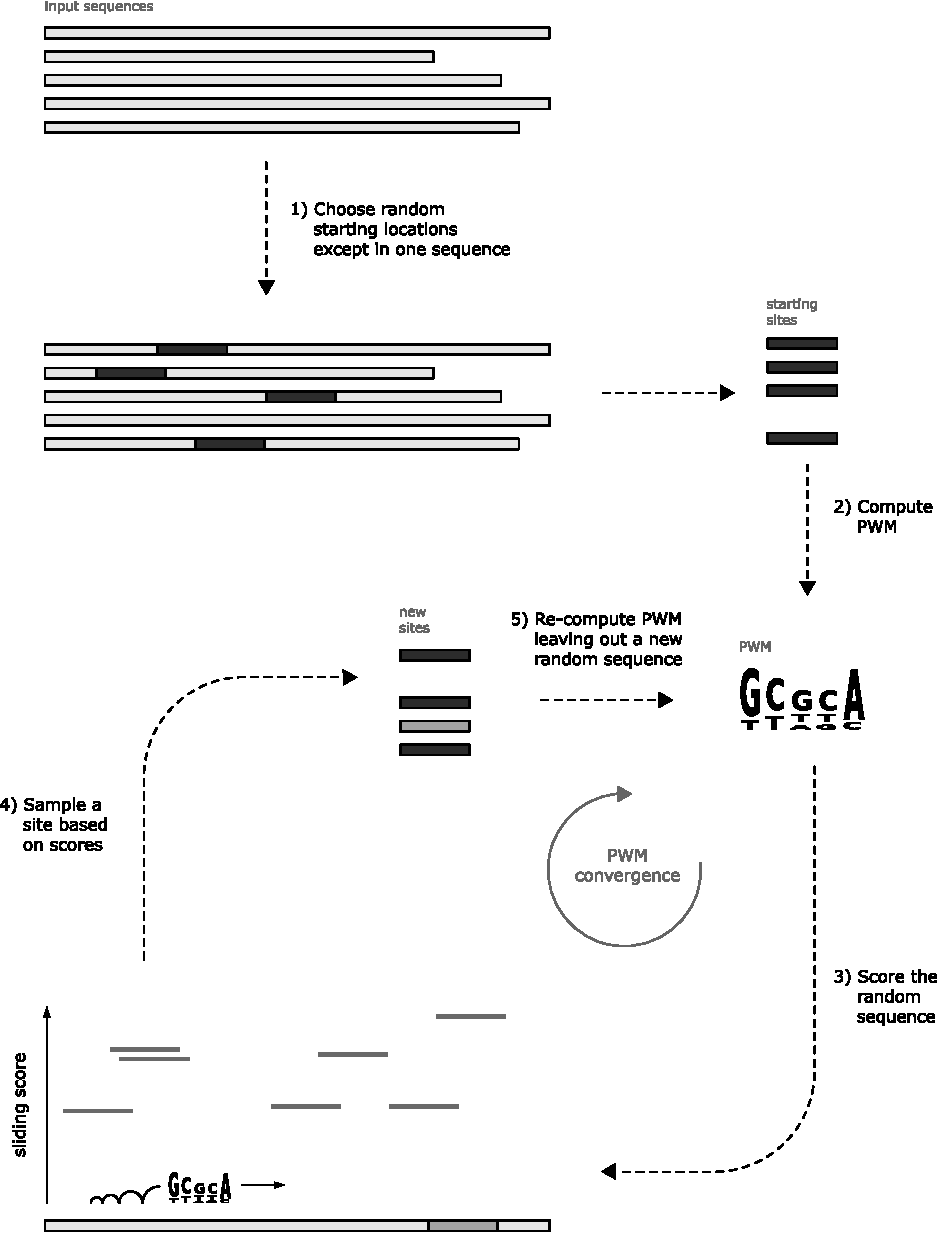
\includegraphics[height=0.80\textheight]{Body/Images-chap1/gibbs.pdf}
\caption[Schematic of the Gibbs sampling algorithm]{Schematic of the
Gibbs sampling algorithm.  As the figure shows, the Gibbs sampling
method is an iterative algorithm that progressively refines a
position weight matrix starting from a random PWM\@.  If the input
sequences contain a very strong motif, Gibbs sampling tends to
converge very quickly upon it.  However, in its original
manifestation~\cite{lawrence1993detecting}, the method was not able
to find motifs that either occurred multiple times in a single
sequence, or were found in some sequences but not others.  In
general, most motif discovery tools using PWMs bear a great deal of
similarity to the original Gibbs sampling method.
 } \label{fig:gibbs}
\end{figure}

Most of the other PWM--based motif discovery tools listed in
Table~\ref{table:pwmMD} use an approach that is similar to the Gibbs
sampler.  In general, these tools excel at finding motifs in DNA
sequences such as cis--regulatory binding sites.
(See~\citet{tompa2005assessing} for an excellent review of this
problem and a demonstration of the power of PWM--based tools.) Other
motif discovery tools use different optimization procedures than the
Gibbs sampler, which are slight variations on the MCMC method, such
as simulated annealing~\cite{kirkpatrick1983optimization} or
expectation maximization. Most of these refinement procedures
guarantee that the algorithm will converge to a
maximum~\cite{gelman1992inference}; however, it is not guaranteed
that a maximum is globally optimal. The optimization can become
trapped in a local optimum, which is called ``slow--mixing'' of the
Markov chain.  New procedures that avoid this are an active area of
study~\cite{liu2001monte}.
